\documentclass[aspectratio=169, 10pt]{beamer}

\usepackage[english]{babel}
% remove this to work with XeTeX
% \usepackage[latin1]{inputenc}  
% \usepackage{lucidabr}  % much nicer than electrum -- DGR 28-Sep-2019
\usepackage{fontspec}     % must use XeTeX with this package
\setmainfont{PT Sans}
% \usepackage[T1]{fontenc}
\usepackage{graphicx} % Allows including images

\usepackage{url} % for live links
\usepackage{xeCJK} % for Chinese text

% -----------
% Set ISRIC style
\usetheme{isric}
% -----------
% Set font to serif - required by the Electrum font
\usefonttheme{serif}

\setcounter{tocdepth}{1}

% -- Section title pages
% Current section
\AtBeginSection[ ]
{
\begin{frame}{Outline}
    \tableofcontents[currentsection]
\end{frame}
}

%----------------
% Title and authors
\title{Soil maps are more than predictors at points and we should evaluate them as such}

%\subtitle{or \ldots point evaluation statistics are not sufficient}

\author{David G.\ Rossiter \& Laura Poggio \hspace{2ex} ISRIC--World Soil
  Information, Wageningen (NL)}

\institute[ISRIC]{ISRIC -- World Soil Information}

\date{22-January-2025 \hspace{2ex} DSM 2025 Bangalore}

%====================================================================
\begin{document}

%----------------
% Title frame

% load background for title 
\setbeamertemplate{background}{ 

\includegraphics[width=\paperwidth,height=\paperheight]
{background_title.png}}

{ \setbeamertemplate{footline}{} % no footer on title
\begin{frame}
\titlepage 
\end{frame} 
}

% load background for all other slides
\setbeamertemplate{background}{

\includegraphics[width=\paperwidth,height=\paperheight]
{background_slides.png}}

\setbeamertemplate{footline}[eawag] % set footer
\addtocounter{framenumber}{-1}  % don't count title page

\begin{frame}{Outline}
    \tableofcontents
\end{frame}

\section{Evaluating Digital Soil Maps -- the problem}

\begin{frame}
\frametitle{Digital Soil Mapping}

Direct production of digital maps\ldots\\
\ldots of soil \textbf{properties} or \textbf{classes}\ldots\\
\ldots by machine-learning or geostatistical methods\ldots\\
\ldots from \textbf{training points}\ldots\\
\ldots and \textbf{covariates} that are surrogates for \textbf{soil-forming factors}, covering the study area.
\\[2ex]
Conceptual basis (McBratney \textit{et al.} 2013): $S = f(s, c, o, r, p, a, n) + \varepsilon$ 
\end{frame}



\begin{frame}
  \frametitle{Example DSM product: ISRIC SoilGrids v2.0 (Poggio \emph{et al.} 2021)}
\begin{figure}
    \centering
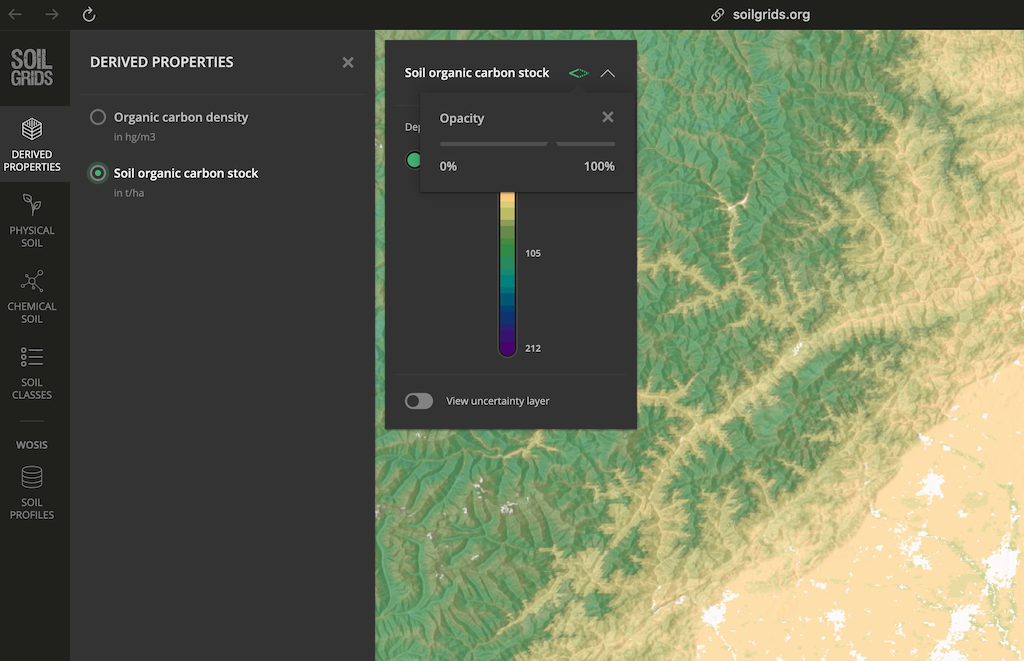
\includegraphics[height=0.75\textheight]{./graphics_david/SoilGrids_SOCstock_Chengdu.png}
\end{figure}
\end{frame}

% \begin{frame}
%   \frametitle{Detail; uncertainty}
% \begin{figure}
% 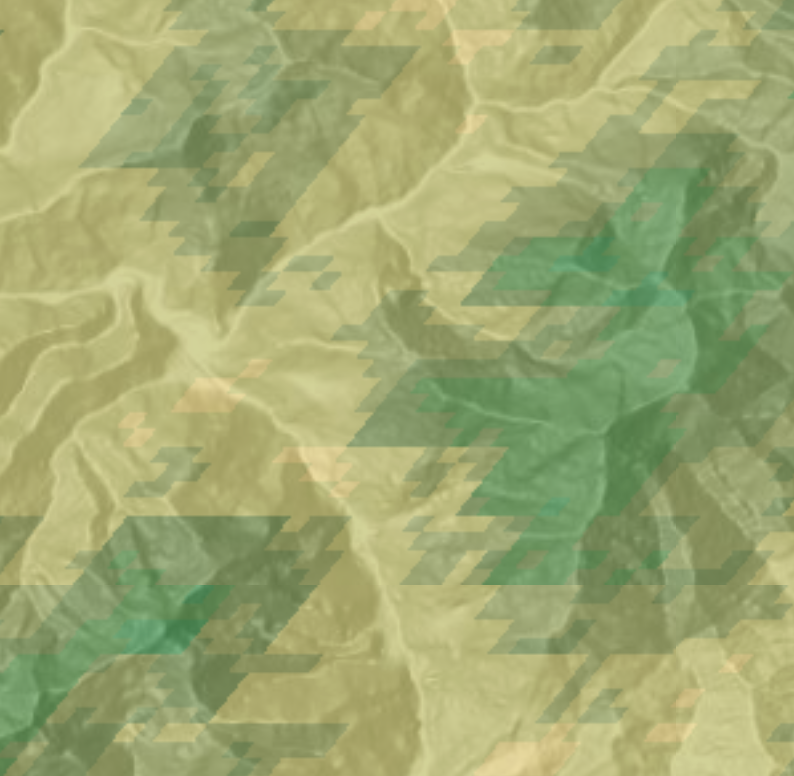
\includegraphics[width=0.4\textwidth]{./graphics_david/SoilGridsDetail.png}
% \hfill
% 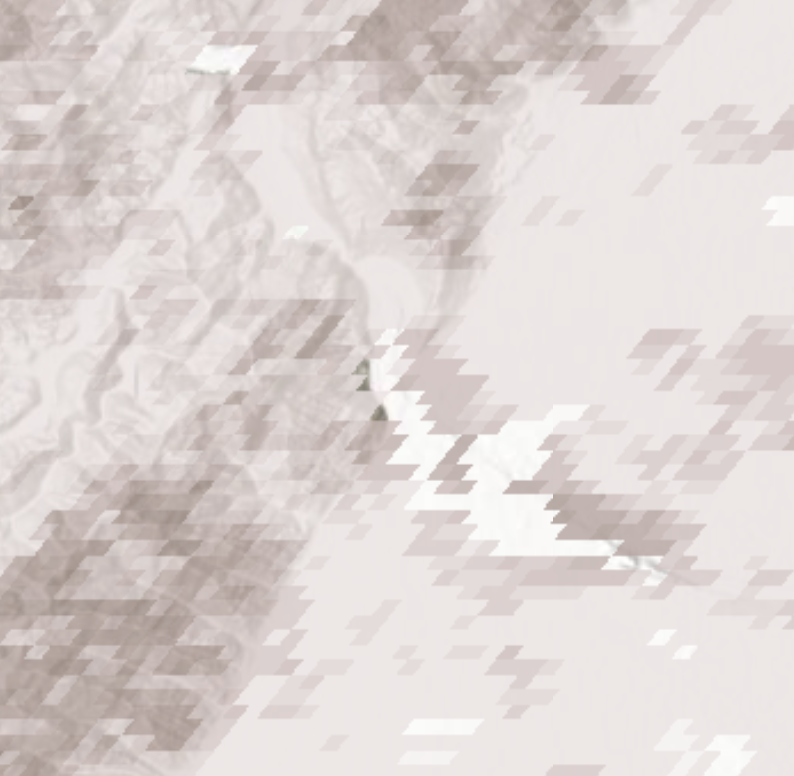
\includegraphics[width=0.4\textwidth]{./graphics_david/SoilGridsUncertainty.png}
% \end{figure}
% \end{frame}

\begin{frame}
  \frametitle{How have these maps been evaluated?}
    \begin{itemize}
        \item On the basis of \textbf{test points}
        \begin{itemize}
            \item independent test set in target area
            \item cross-validation of out-of-bag (OOB) observations in Machine Learning (ML) methods
            \item repeated splits into test/training of one dataset
        \end{itemize}
      \item (pointwise) \textbf{evaluation statistics}
        \begin{itemize}
        \item ME, RMSE
        \item 1:1 $R^2$ (MCC, Nash-Sutcliffe Model
          Efficiency)
        \item gain/bias of actual regressed on observed
        \item \ldots
        \end{itemize}
    \end{itemize}
\end{frame}


\begin{frame}
  \frametitle{Problems with evaluation by point statistics -- Internal}
From the \textbf{mapper's} point of view:
\begin{enumerate}
    \item Based on a \textbf{limited number of observations}, far fewer than the number of predictions (grid cells, ``pixels'').
    \item Evaluating at \textbf{points}, but predicted value is for the \textbf{grid cell} (either centre or block average)
    \item Evaluation points are almost never from an independent  \textbf{probability sample}.
  \item Cross-validation and data-splitting approaches rely on this \textbf{biased} point set.
  \item \textbf{Evidence}: Different DSM approaches can result in maps    with quite \textbf{similar ``validation statistics''} but obviously \textbf{different spatial patterns}.
  \end{enumerate}
\end{frame}


\begin{frame}
  \frametitle{ISRIC WoSIS: limited, non-probability evaluation points}
\begin{figure}
    \centering
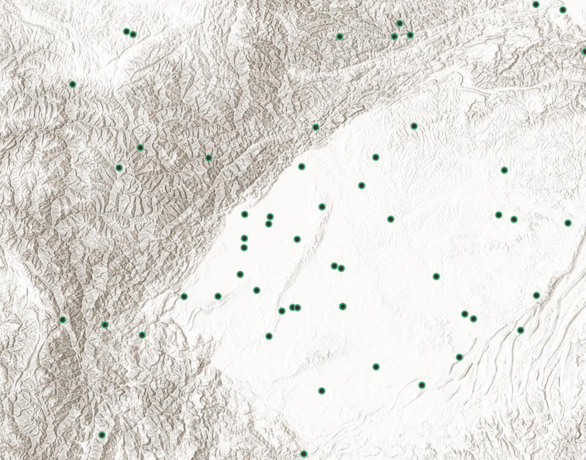
\includegraphics[height=0.65\textheight]{./graphics_david/SoilGridsProfiles_Chengdu.png}
\end{figure}
\end{frame}

% \begin{frame}
%   \frametitle{\emph{Different} ML methods, covariates,  points}
%     \begin{figure}
%         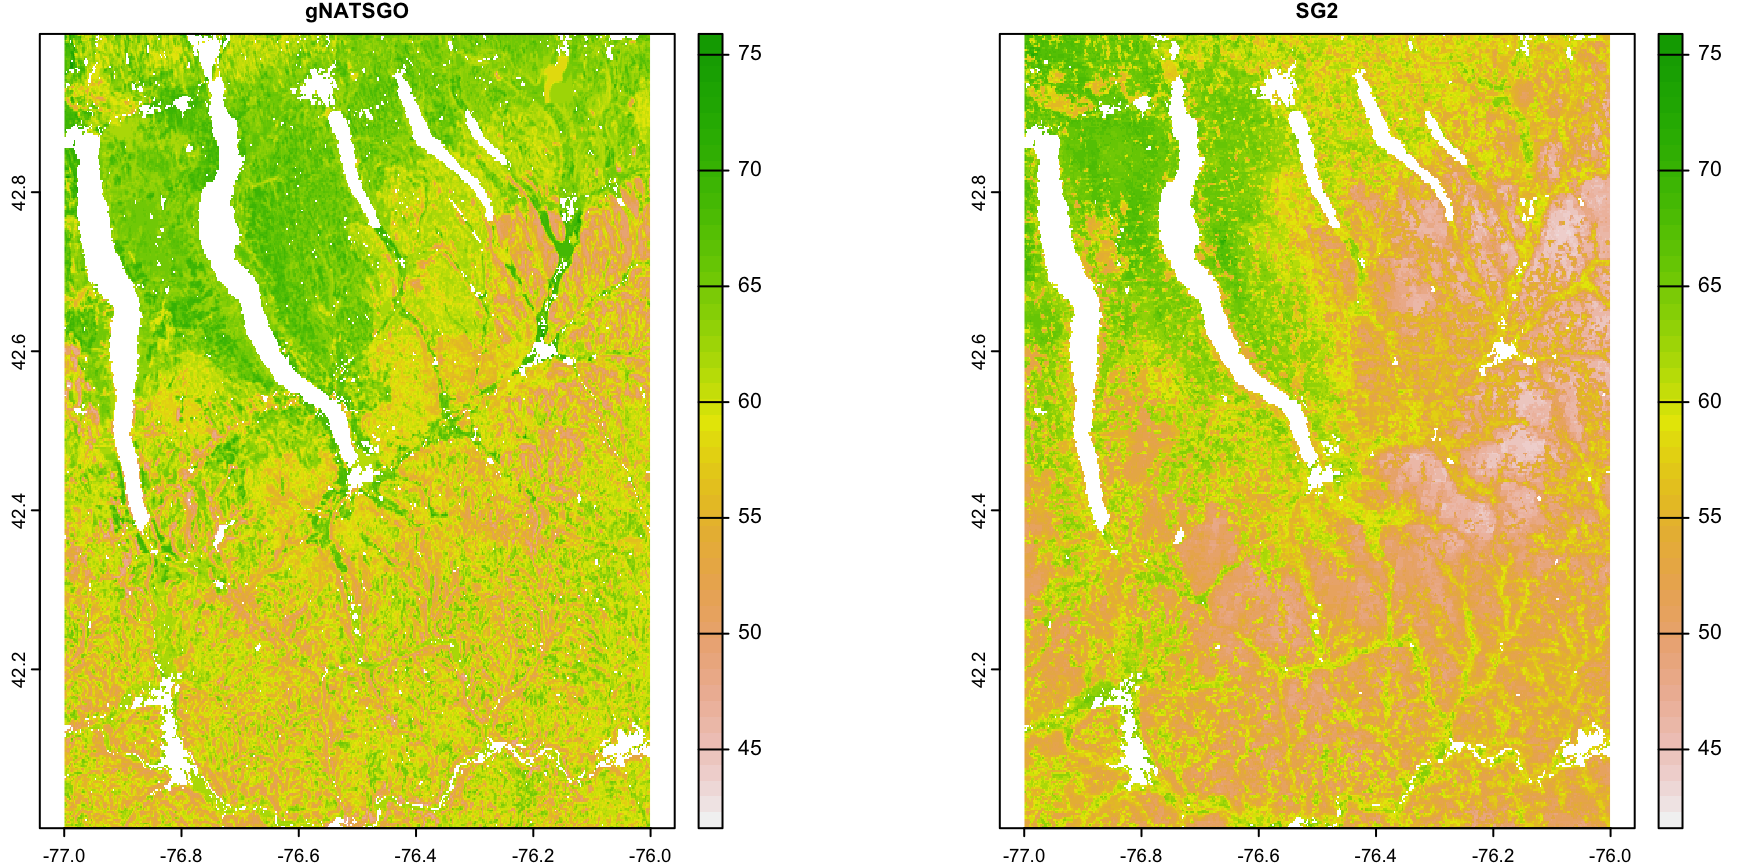
\includegraphics[width=0.49\linewidth]{./graphics_david/Fig07a.png}
%         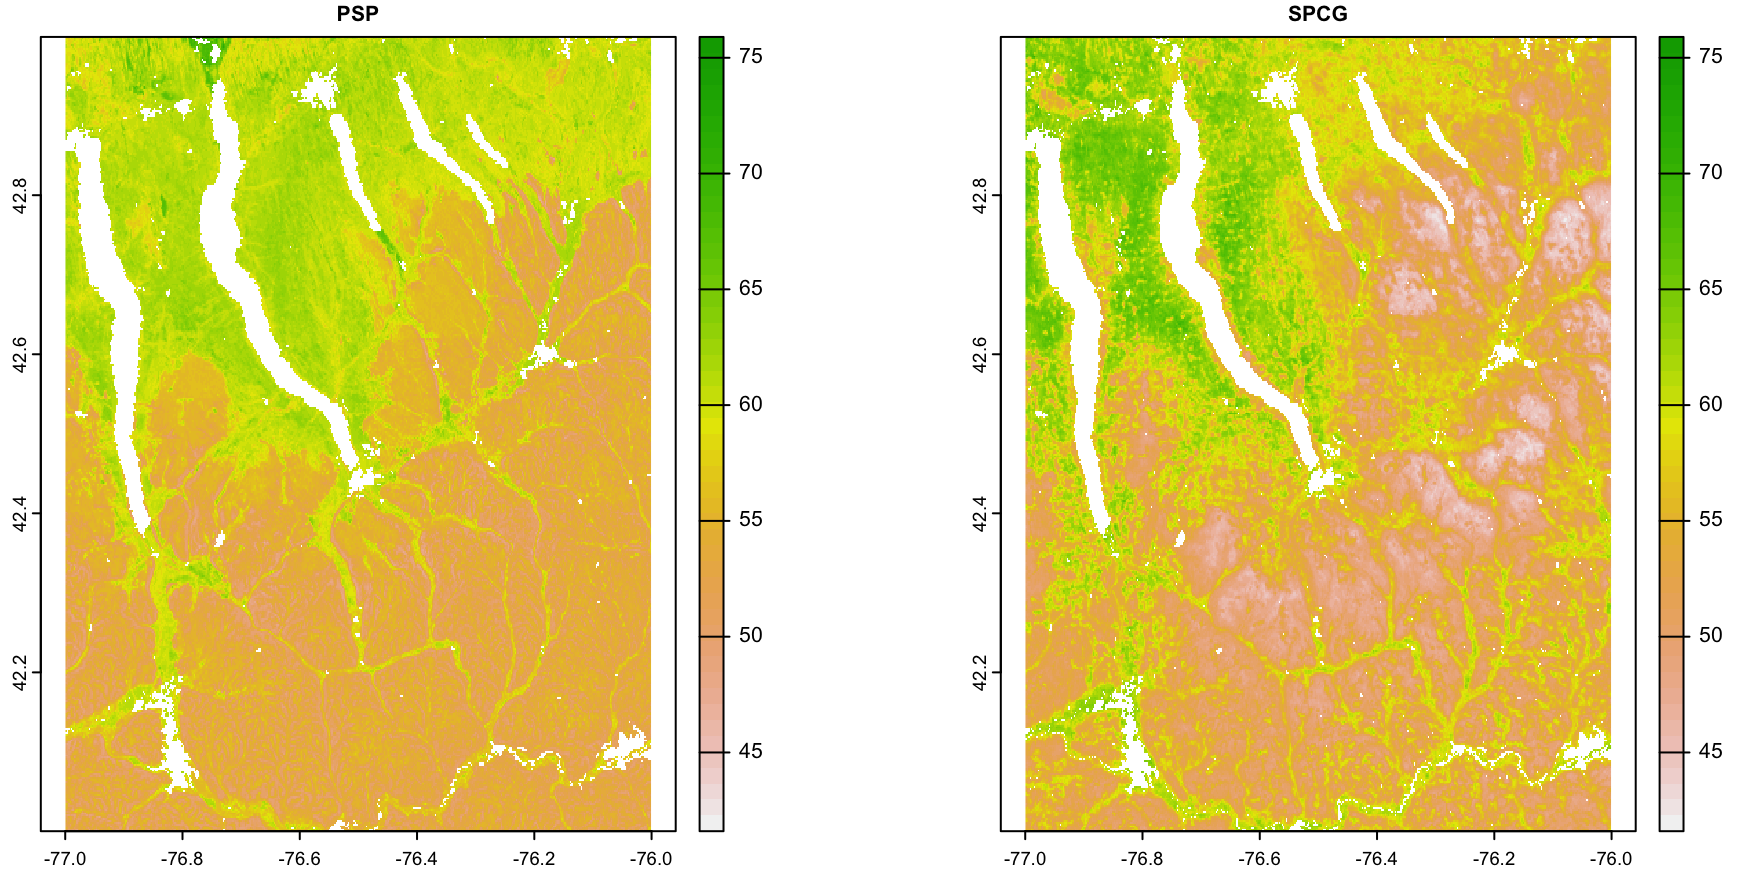
\includegraphics[width=0.49\linewidth]{./graphics_david/Fig07b.png}
% \par        
%     Central NY State (USA), pH x 10, 0-5~cm; from Rossiter \emph{et al.} (2022)
%     \end{figure}
%  Some obvious difference in \textbf{values} but also \textbf{patterns}.
% \end{frame}

\begin{frame}
  \frametitle{\emph{Same} ML method, covariates, points; different
    \emph{parameters}}
    \begin{figure}
        \centering
        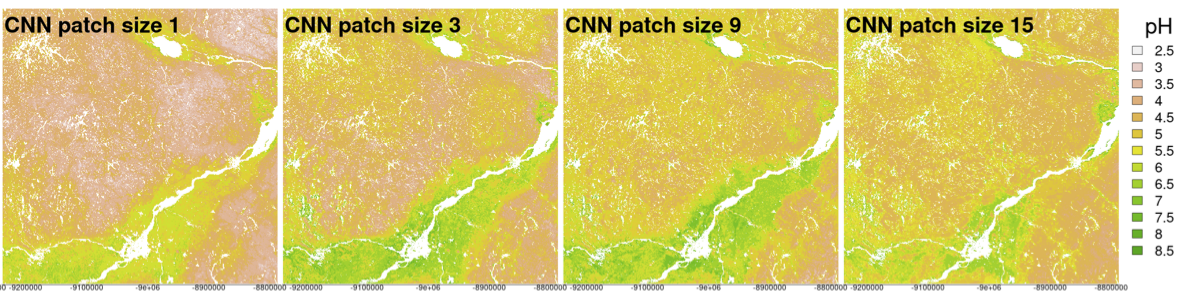
\includegraphics[width=\textwidth]{./graphics_david/GenovaPosterFig1a.png}
        \par Montr\'{e}al area, PQ, pH 0-5~cm
    \end{figure}
{Convolutional Neural Network (CNN), different window size (Giulio Genova, ISRIC)}
\end{frame}

\begin{frame}
  \frametitle{Almost \emph{identical} evaluation statistics}
    \begin{figure}
        \centering
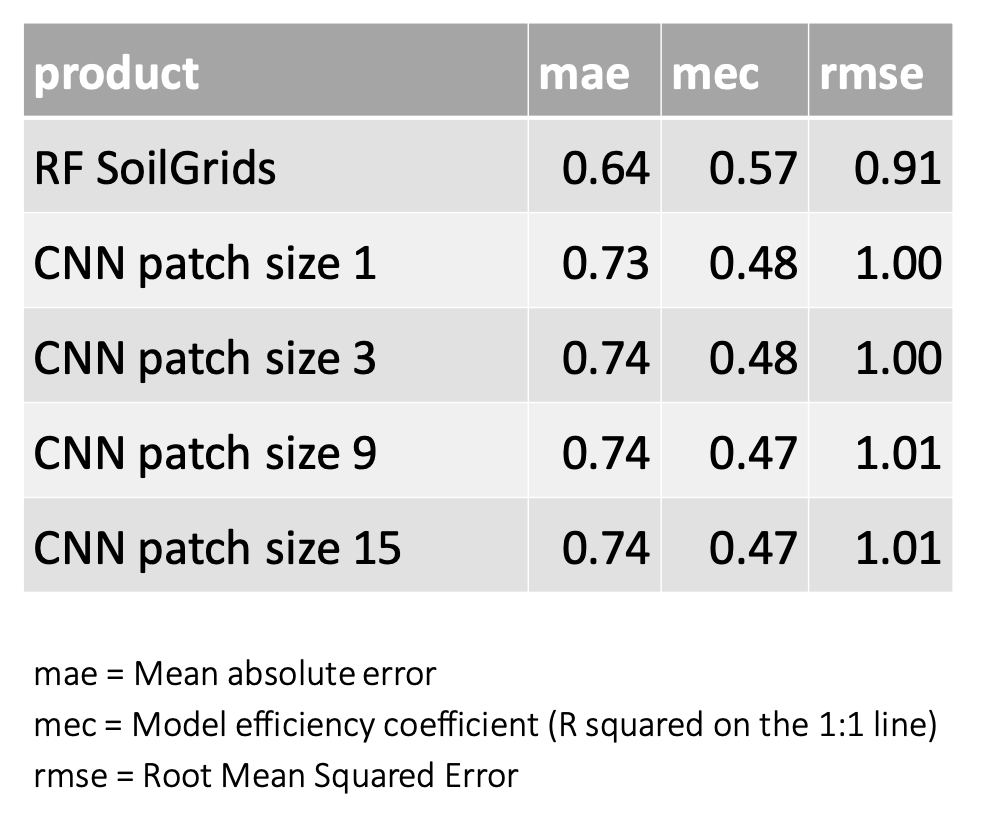
\includegraphics[height=0.7\textheight]{./graphics_david/Genova_poster_stats.png}
\end{figure}
\end{frame}


% \begin{frame}
%   \frametitle{Different surveys, different patterns -- which is better?}
%     \begin{figure}
%         \centering
%         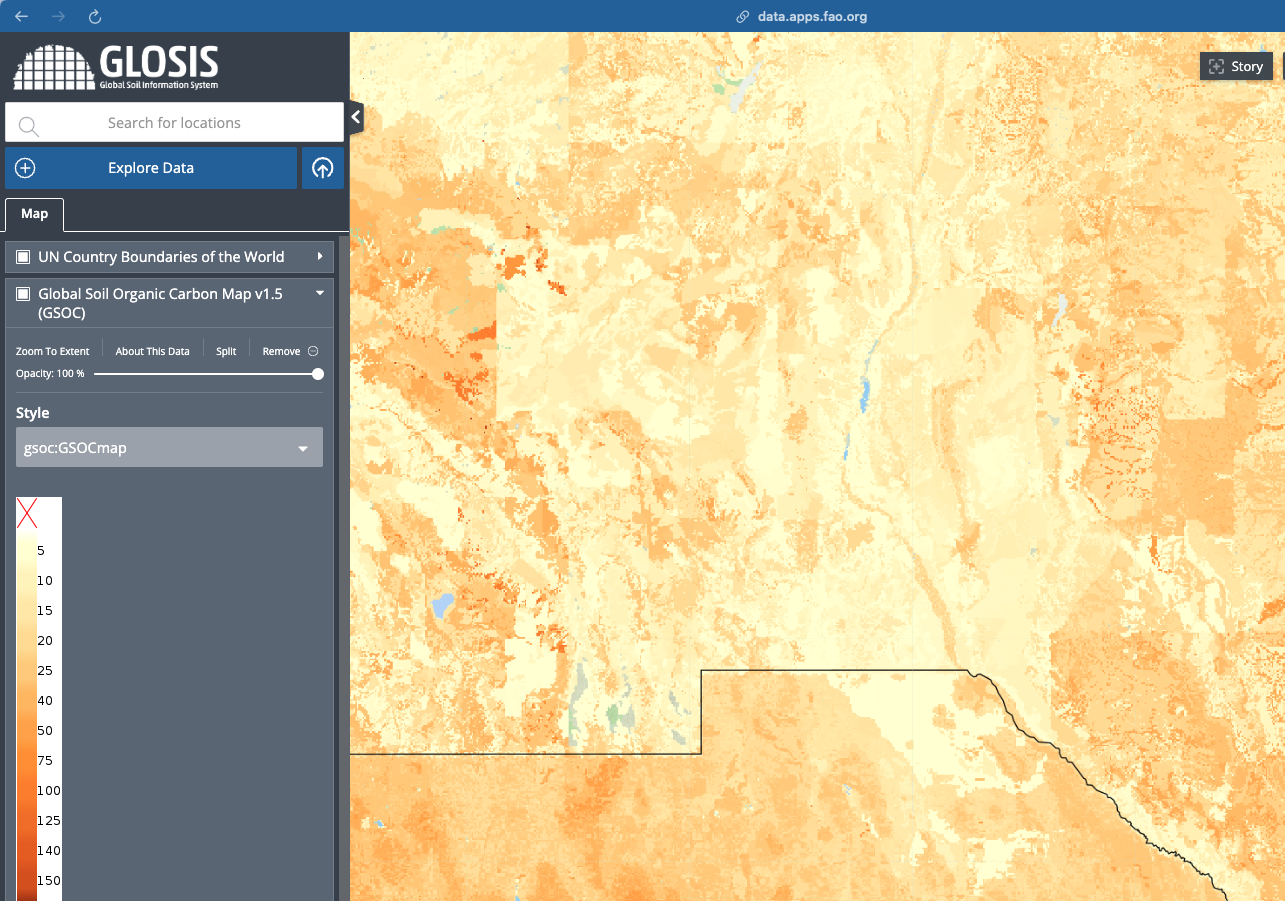
\includegraphics[height=0.6\textheight]{./graphics_david/GLOSIS_SOC_LasCrucesRegion.png}
%      \end{figure} 
% \end{frame}


\begin{frame}{Problems with evaluation by point statistics -- External}

From the \textbf{map user's} point of view:
\begin{enumerate}
\item  Soils are \textbf{managed as units} at some scale, \emph{not} point-wise.
\item  Land-surface models often rely on 2D or 3D \textbf{connectivity} between grid cells.
  \begin{itemize}
  \item Especially hydrology / chemical transport models
  \end{itemize}
\item  Fieldwork shows that \textbf{soils  occur in more-or-less homogeneous patches}, \emph{not} as isolated
  pedons (Fridland, Boulaine, Hole \ldots).
\item How to identify \textbf{artefacts} resulting from the DSM model?
  \end{enumerate}
  
\end{frame}

\begin{frame}
  \frametitle{Legacy map updated by DSM -- realistic or artefacts?}
    \begin{figure}
        {\centering
        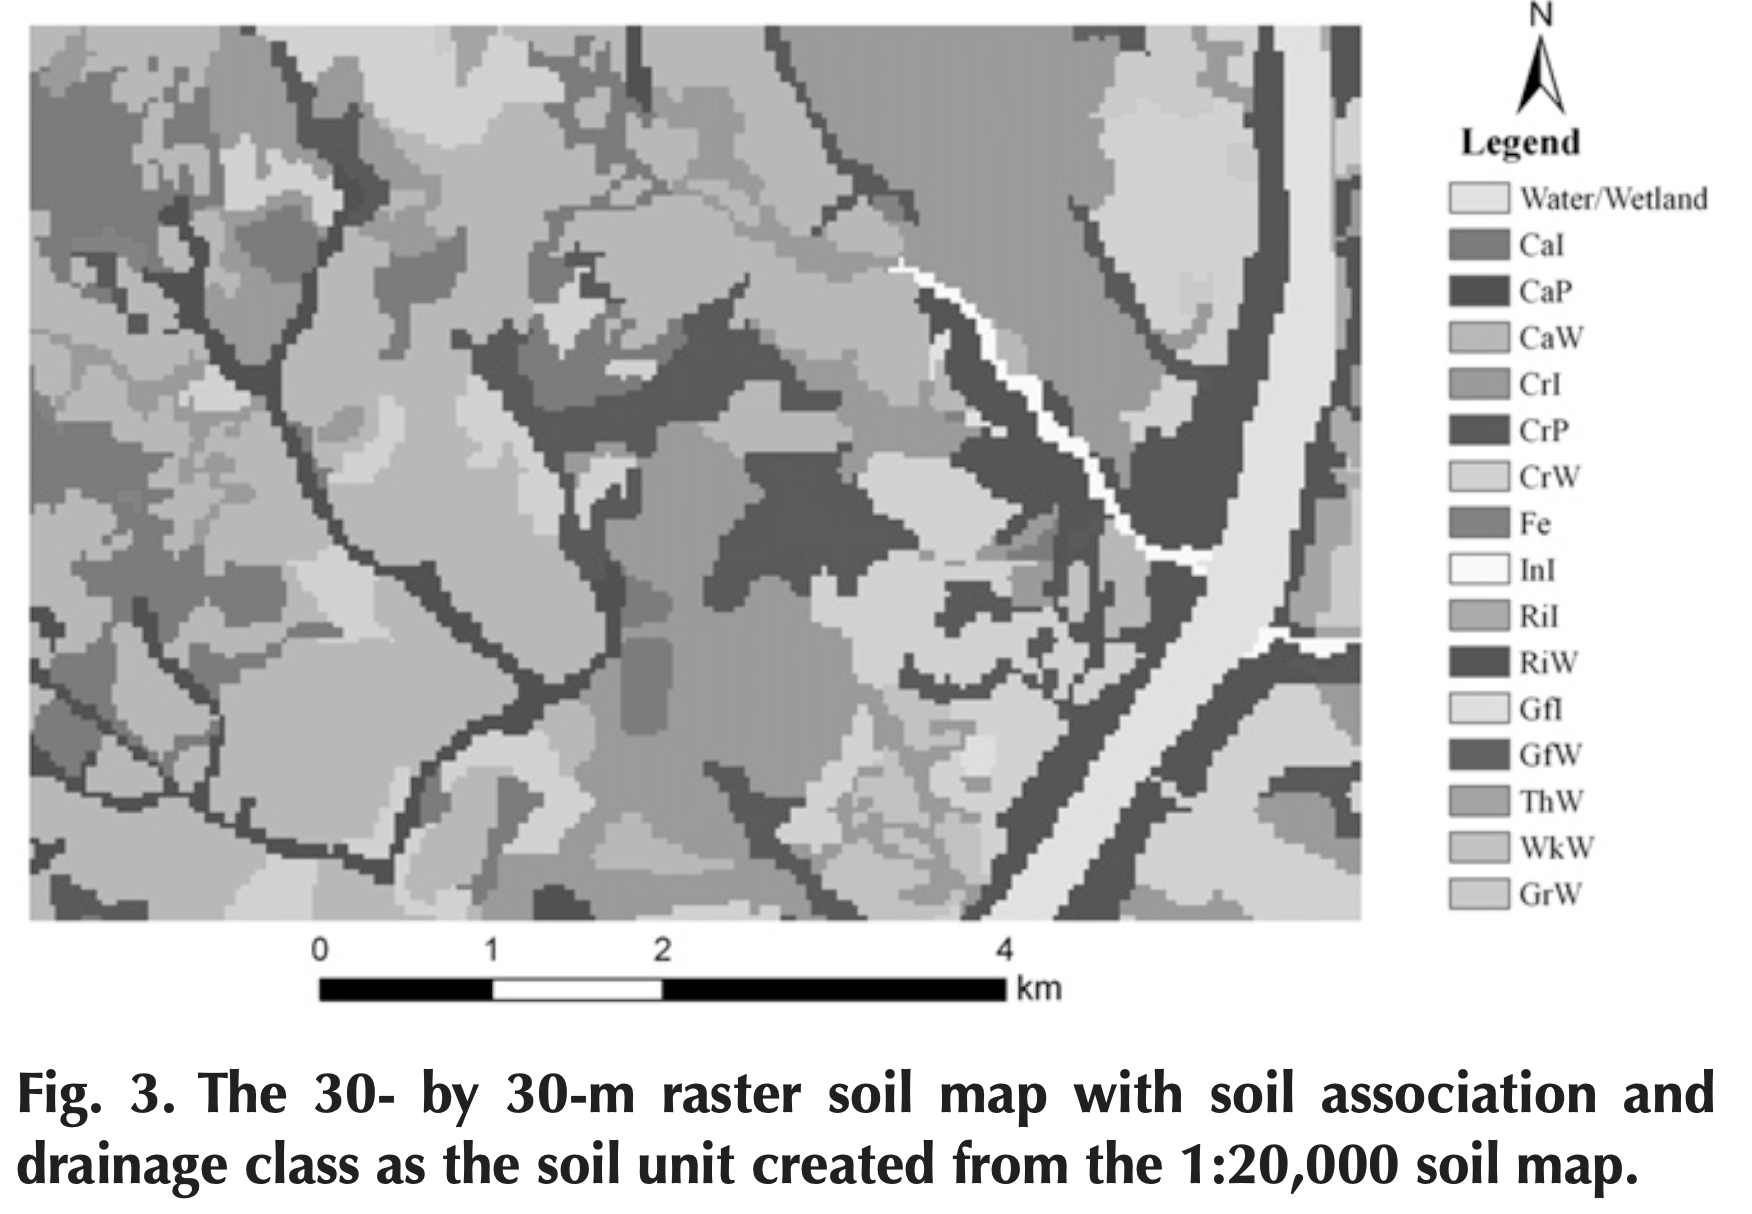
\includegraphics[width=0.48\textwidth]{./graphics_david/sssaj2010.0002_YL_original.png}
        \hfill
        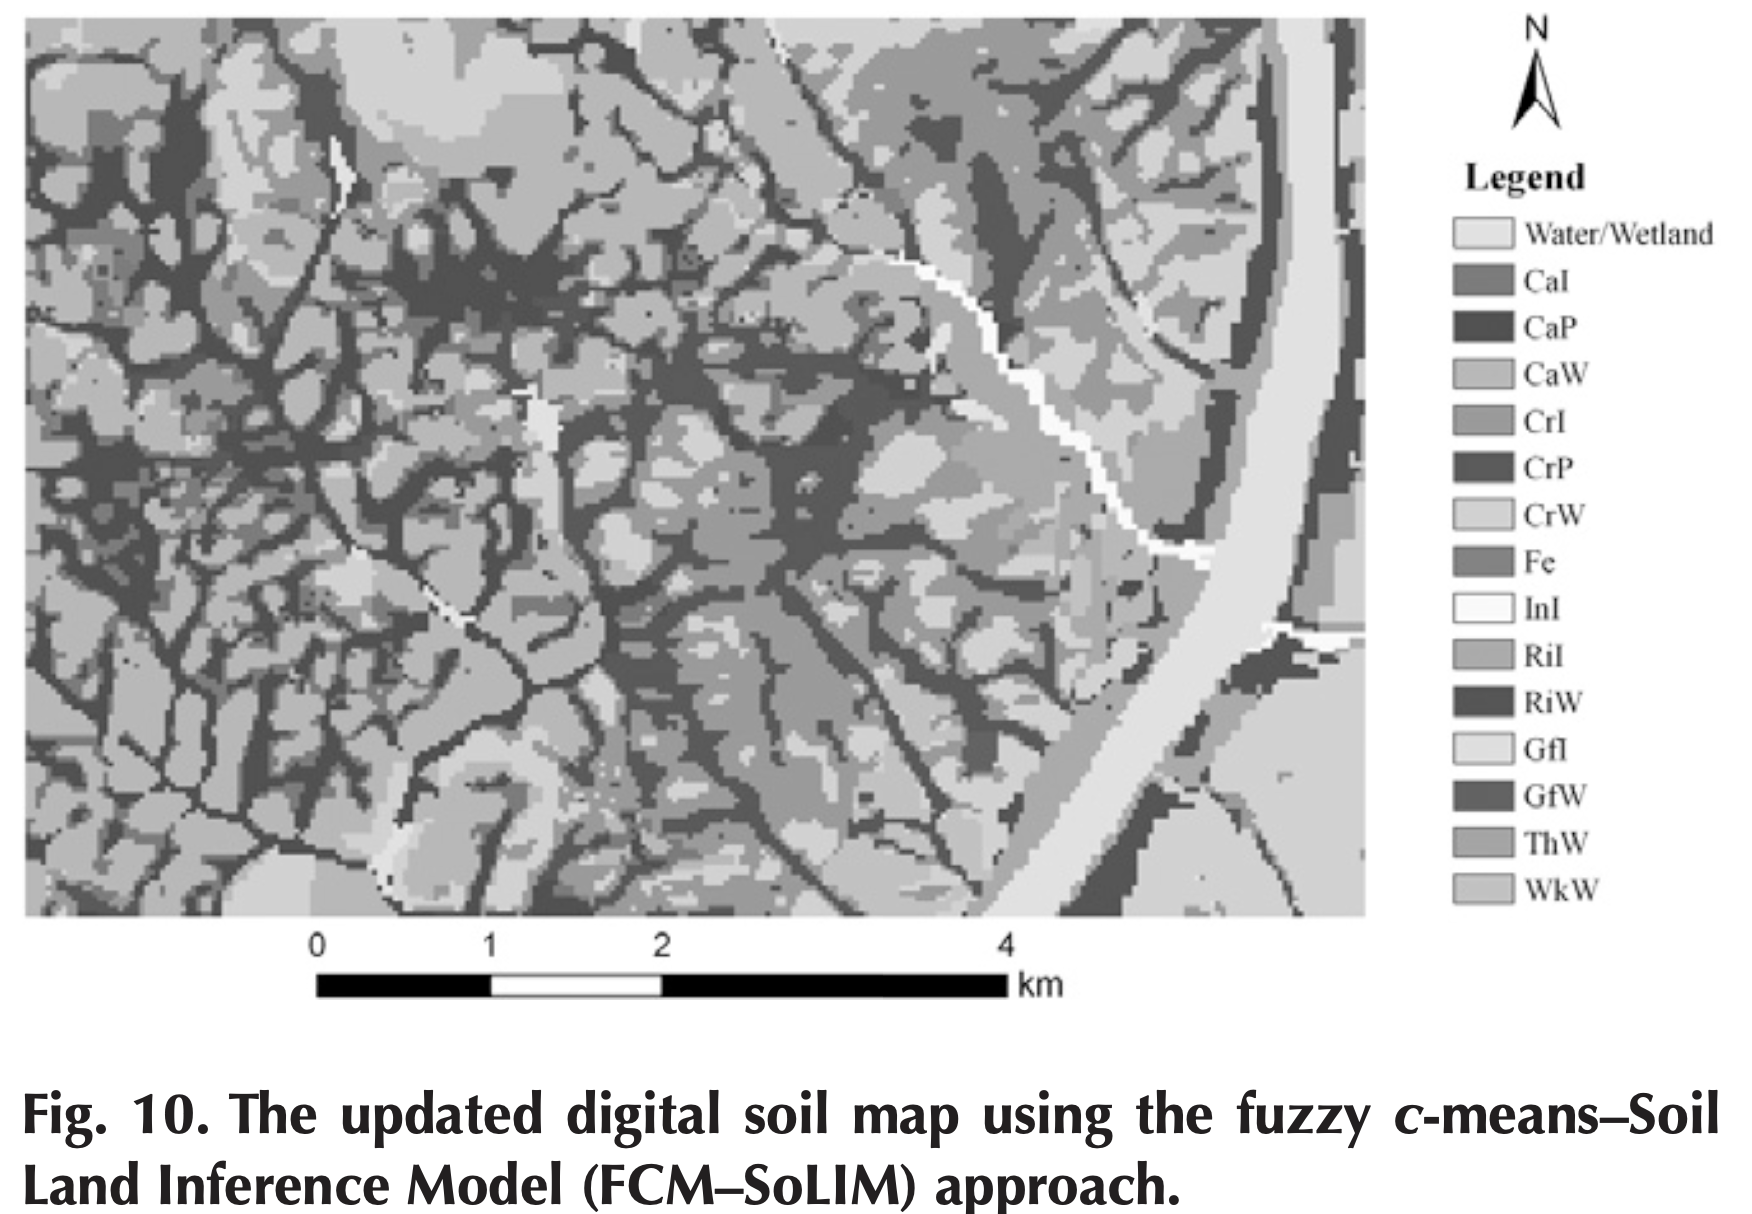
\includegraphics[width=0.48\textwidth]{./graphics_david/sssaj2010.0002_YL_updated.png}
        }\\\flushleft(L. Yang 杨琳 \emph{et al.} 2010)  
    \end{figure}
\end{frame}


\section{Pattern analysis}

\begin{frame}{Pattern analysis}
    \begin{itemize}
        \item \textbf{Quantitative} description of (spatial) patterns
        \item Long history in \textbf{image analysis} and \textbf{landscape ecology}
        \item Applied to landscape mosaics (FRAGSTATS)
        \item R packages  \texttt{motif}, \texttt{landscapemetrics}, \texttt{rassta}, \texttt{superpixels} (\textbf{aggregation})
        \item Unix program \texttt{geoPAT2}\footnote{\url{https://github.com/Nowosad/geopat2}} (\textbf{segmentation})
   \end{itemize}
\end{frame}

\begin{frame}{Levels of pattern analysis}
\begin{enumerate}
    \item \textbf{Characterize} the pattern of one map
    \item \textbf{Compare} patterns of several maps
    \item \textbf{Aggregate} or \textbf{Segment} map by its patterns -- let the map ``speak for itself''
    \item \textbf{Evaluate} pattern with respect to ``reality''
\end{enumerate}
\end{frame}

\subsection{Continuous soil properties maps}

\begin{frame}{Characterizing patterns -- \emph{continuous} soil properties}
    \begin{enumerate}
        \item \textnormal{Variogram analysis}: inherent spatial scales and variability averaged over entire map
        \item \textbf{Moving-window autocorrelation}: how does this vary across the DSM?
          \begin{itemize}
          \item Shows ``hot spots'' of high local consistency (high  values of Moran's \textit{I}), ``cold spots'' of high local  variability (low values)
          \item Do these correspond with perceived local variability?
          \end{itemize}
    \end{enumerate}
\end{frame}

\begin{frame}{Variograms with fitted models}
    \begin{figure}
        \centering
        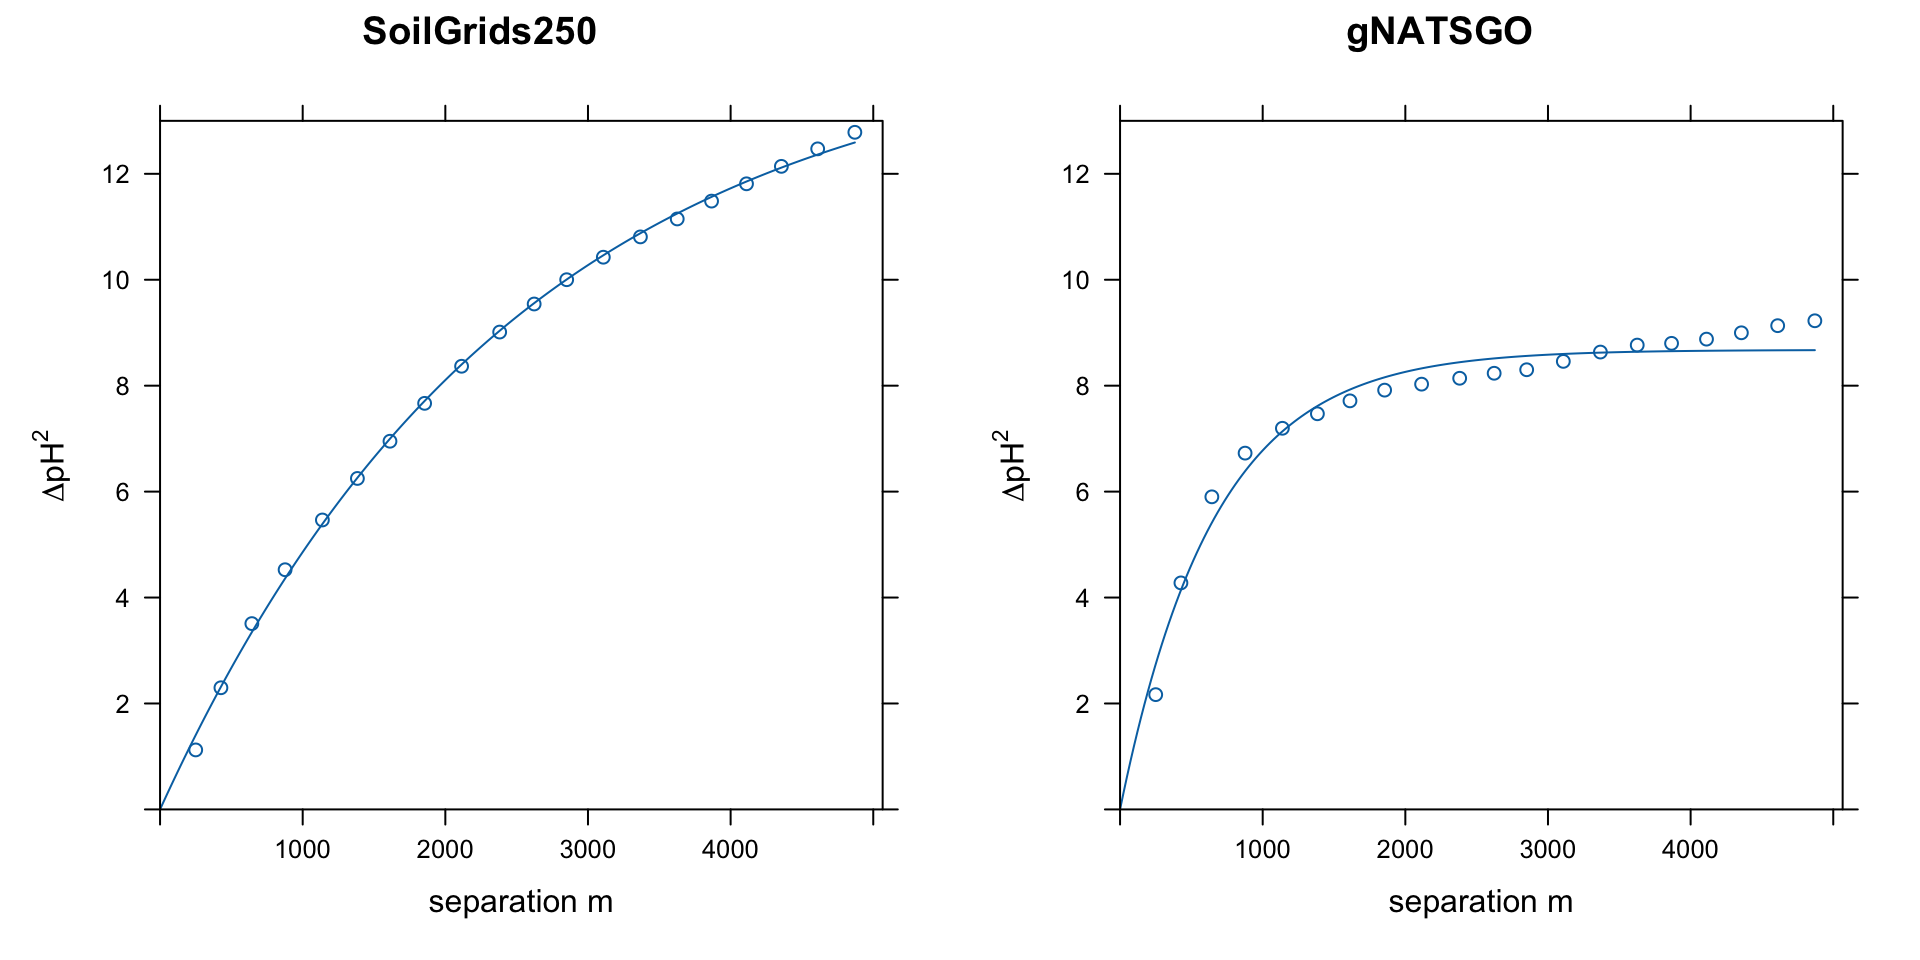
\includegraphics[height=0.6\textheight]{./graphics_david/variograms.png}
        \\${(\mathrm{pH} * 10)}^2$; interpret sill and range
    \end{figure}
\end{frame}

\begin{frame}{Moving-window autocorrelation}
    \begin{figure}
        \centering
        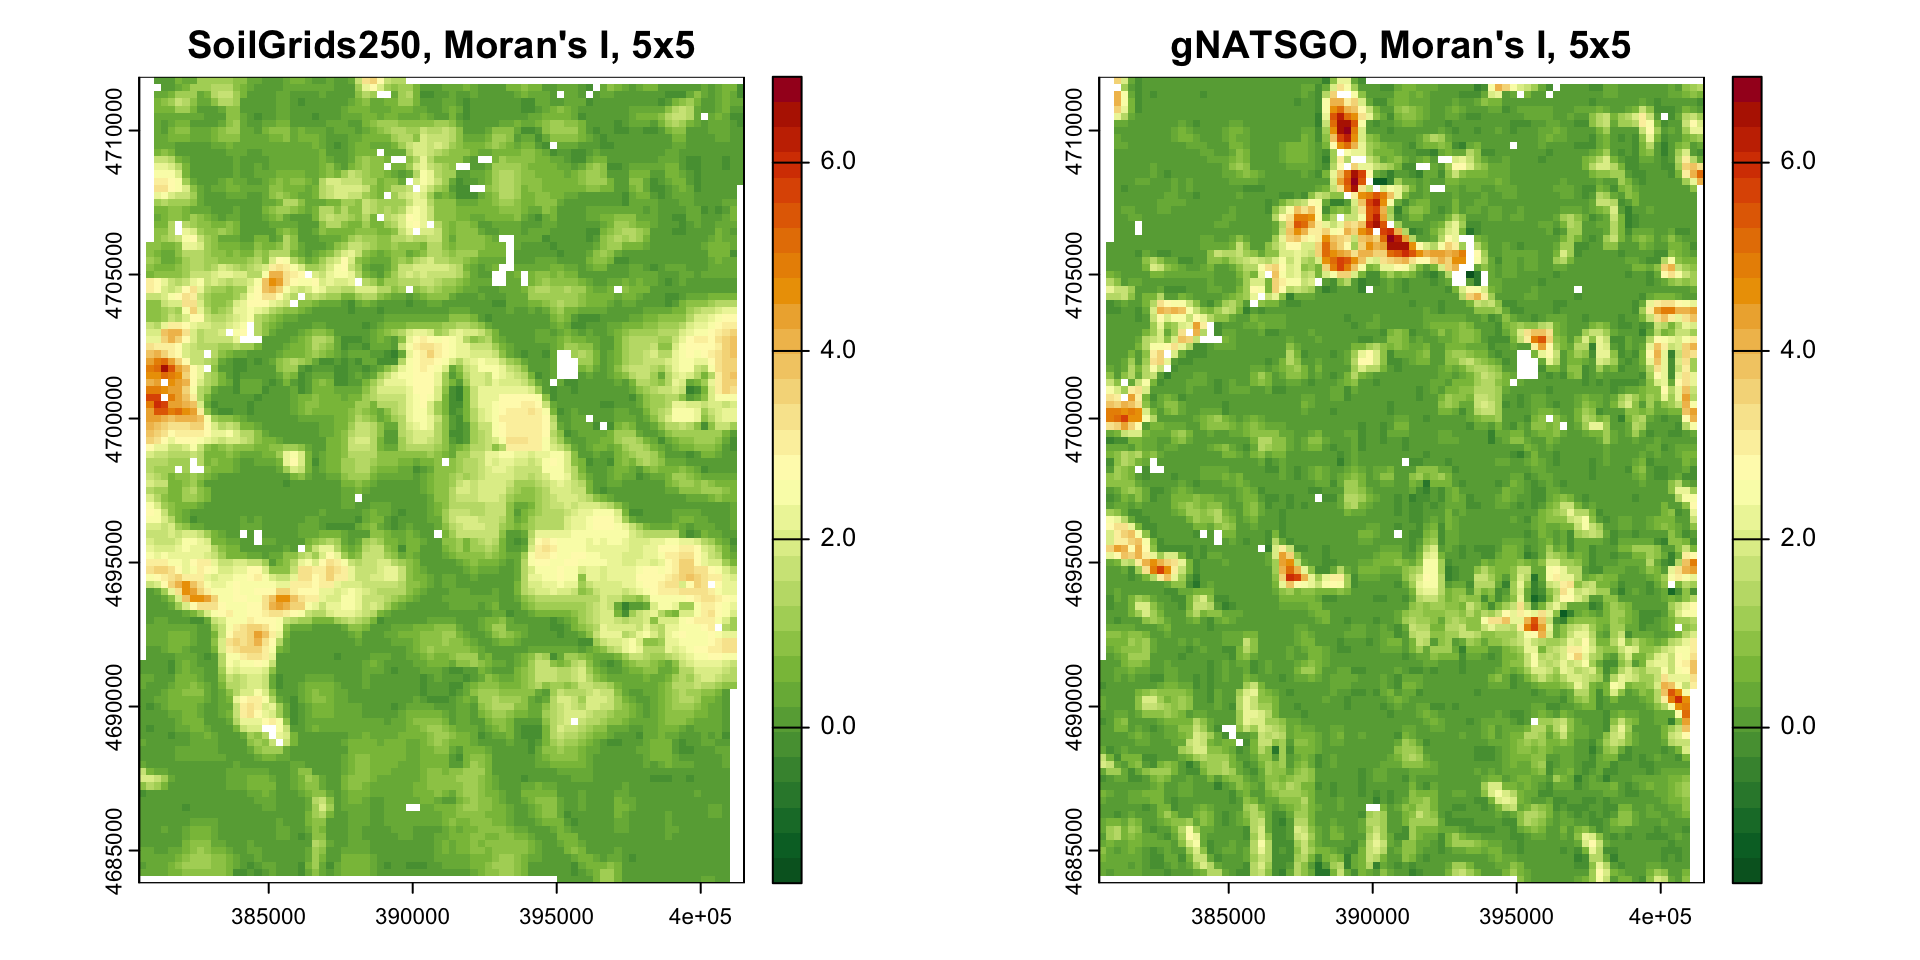
\includegraphics[height=0.6\textheight]{./graphics_david/moving-window-5-1.png}
    \end{figure}
%
    high values of Moran's \textit{I}: high local spatial correlation (consistent values)
\end{frame}

\subsection{Class or classified maps}

\begin{frame}{Characterizing patterns -- \emph{classified} soil properties or soil \textbf{classes}}
\begin{itemize}
    \item Well-known techniques from landscape ecology (FRAGSTATS)
    \item Select metrics that are relevant to the objective
    \begin{itemize}
        \item here, characterizing the soil pattern
    \end{itemize}
    \item For continuous properties must \textbf{slice} (discretize)
    \begin{itemize}
        \item \textbf{meaningful limits} for an application (e.g., pH for liming recommendation), or \ldots
        \item equal-intervals, or \ldots
        \item histogram equalization
    \end{itemize}
\end{itemize}
\end{frame}

% \begin{frame}{Histogram equalization of pH~x~10 into 8 classes}
%     \begin{figure}
%         \centering
% 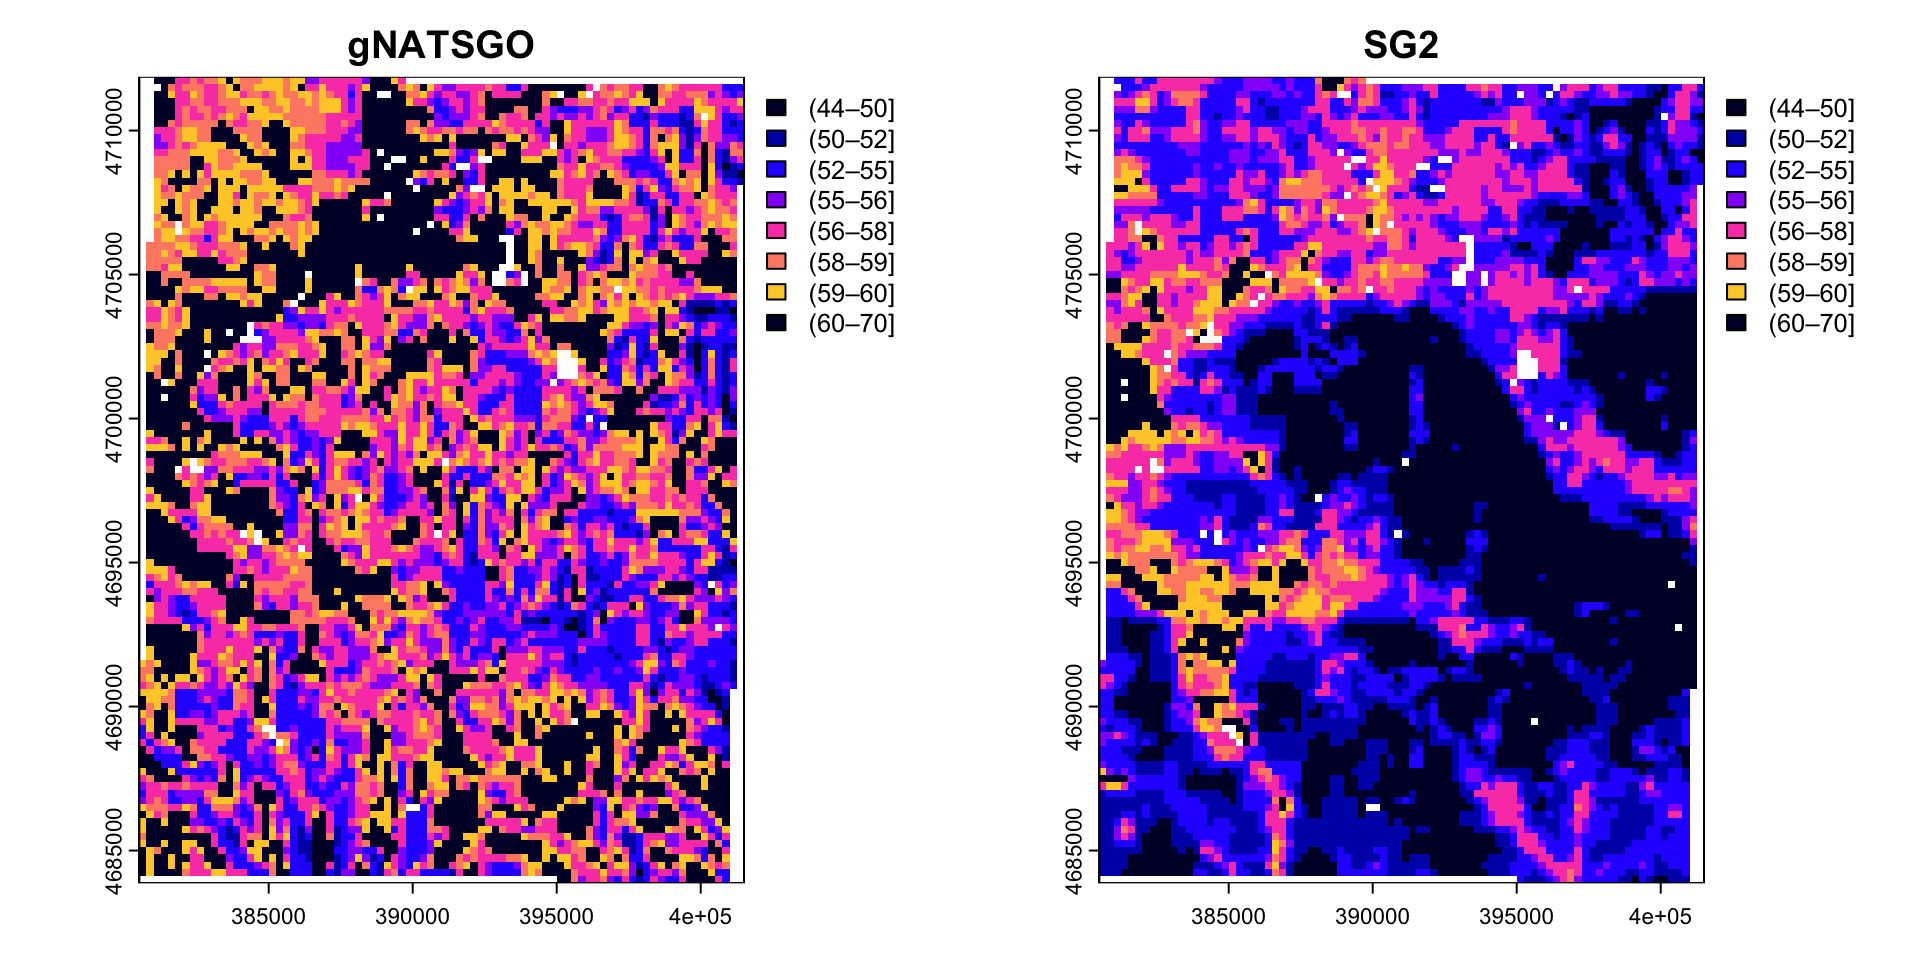
\includegraphics[height=0.8\textheight]{graphics_david/show.classified-1.png}
%     \end{figure}
% \end{frame}

\begin{frame}{Some useful metrics}
\begin{itemize}
    \item \texttt{LAI}   \emph{landscape aggregation}: index quantifies how \textbf{connected} is each class, averaged over all classes
    \item \texttt{MFD} \emph{mean fractal dimension}: describes multi-scale \textbf{patch complexity}
    \item \texttt{LSI} \emph{landscape shape index}: quantifies the \textbf{complexity of the patch shapes}
    \item \texttt{SHDI} \emph{Shannon diversity index}: a measure of (1) the \textbf{legend complexity}, (2) the \textbf{(un)balance} between classes
    \item \texttt{GLCM} \emph{Gray Level Co-occurrence Matrix}: characterizes the ``texture'' of a raster class map
      \begin{itemize}
      \item \textbf{local} statistical properties of a window as it moves across the map.
      \end{itemize}
    \item \texttt{COVE} \emph{Co-occurrence vector}: summarizes the adjacency structure
\end{itemize}    
\end{frame}

% \begin{frame}{Metric: landscape aggregation index}

% This quantifies how \textbf{connected} is each class, averaged over all classes.
%     $$\mathrm{LAI} = \Bigg[∑_{i=1}^m \Big( \frac{g_{ii}}{max-g_{ii}} \Big) P_{i} \Bigg](100)$$
    
%     where $g_{ii}$ is the number of like adjacencies, $(\mathrm{max}-g_{ii})$ is the classwise maximum possible number of like adjacencies of class $i$
% \par
%     \textbf{Low} values: classes are \textbf{scattered} over the map; \textbf{high} values: classes tend to \textbf{clump} together
% \end{frame}

% \begin{frame}{Metric: mean fractal dimension}

% A shape metric, describing multi-scale patch complexity.
% $$\mathrm{FRAC} = \frac{2 * \ln * (0.25 * p_{ij})} {\ln a_{ij}}$$ 

% where the patch perimeters are ${p_{ij}}$ in linear units and the areas are ${a_{ij}}$ in square units.
% \\
% This measures the intricacy of the soil pattern.

% \end{frame}

% \begin{frame}{Metric: landscape shape index}
%     This quantifies the \textbf{complexity of the patch shapes}, across the map.
%     $$   \mathrm{LSI} = \frac{0.25 E'}{\sqrt{A}}$$

%     where $A$ is the total area of the landscape and $E'$ is the total length of edges, including the boundary.
% \end{frame}

\begin{frame}{Example metric: Shannon diversity index}
  \par
  This measures both the number of classes and their relative abundance.\\[2ex]
  It is a measure of (1) the \textbf{legend complexity}, (2) the \textbf{(un)balance} between classes.
    $$ D = - \sum_{i=1}^N p_i \ln p_i$$
  \par
    where $p_i$ is the proportion of pixels of class $i = (1 \ldots N)$
\end{frame}

% \begin{frame}{Example metric: Co-occurrence vector}
%   \begin{itemize}
%   \item 
%     Summarizes the entire \textbf{adjacency structure} of a map.% as a  normalized co-occurrence matrix: which classes are spatially adjacent to each other?
%   \item
%     This is a probability vector for the \textbf{spatial co-occurrence} of  different   classes in the map.
%     \begin{itemize}
%     \item e.g., different soil classes -- do we expect Histosols next to Vertisols?
%     \item e.g., different classes of a classified property -- do we expect abrupt changes of pH class?
%     \end{itemize}
%  %   \item
% %    The ``distance'' between co-occurrence vectors from two maps can be computed   as a measure of the (dis)similarity between these structures
% %    (Jensen-Shannon distance, used to compare probability distributions)
%   \end{itemize}
% \end{frame}


\begin{frame}{Comparing maps with these metrics}
\par
    % latex table generated in R 4.2.1 by xtable 1.8-4 package
% 
\begin{tabular}{llllll}
  \hline
product & ai & frac\_mn & lsi & shdi & shei \\ 
  \hline
gNATSGO & 48.188 & 1.034 & 22.602 & 1.666 & 0.801 \\ 
  SG2 & 50.659 & 1.034 & 21.768 & 2.06 & 0.991 \\ 
  SPCG & 58.483 & 1.041 & 18.557 & 1.887 & 0.907 \\ 
  PSP & 47.025 & 1.04 & 23.232 & 1.898 & 0.913 \\ 
   \hline
\end{tabular}

      \\[1.5ex]
      Landscape metrics statistics, pH 0--5~cm (top); 30--60~cm (bottom).
      \\[1.5ex]
      \texttt{frac\_mn}: Mean Fractal Dimension; \texttt{lsi}: Landscape Shape Index; \texttt{shdi}: Shannon Diversity; \texttt{shei}: Shannon Evenness; \texttt{ai}: Aggregation Index\\[1.5ex]
      (Evaluation area: -77---76\textdegree~E, 42--43\textdegree~N)
\end{frame}

% \begin{frame}{V-measure (Nowosad \& Stepinski 2018)}
% \begin{itemize}
%     \item Compares \textbf{different spatial partitions} into classes
% \item Two maps could have the same \textbf{total areas} of each class, and even the same \textbf{number of polygons} within each class, and even the same \textbf{size distribution} of these polygons \ldots
% \item \ldots and yet be completely different in \textbf{how they partition space} into classes.
% \item \textbf{homogeneity}: variance of the regions within a zone, normalized by the variance of the regions in the entire domain of the \textbf{first} map
% \item \textbf{completeness}: variance of the zones within a region, normalized by the variance of the zones in the entire domain of the \textbf{second} map.
% \item $V = \frac{h \times c}{h + c}$
% \end{itemize}
% \end{frame}

% \begin{frame}{Comparing two maps with V-measures}
%     \begin{figure}
%         \centering        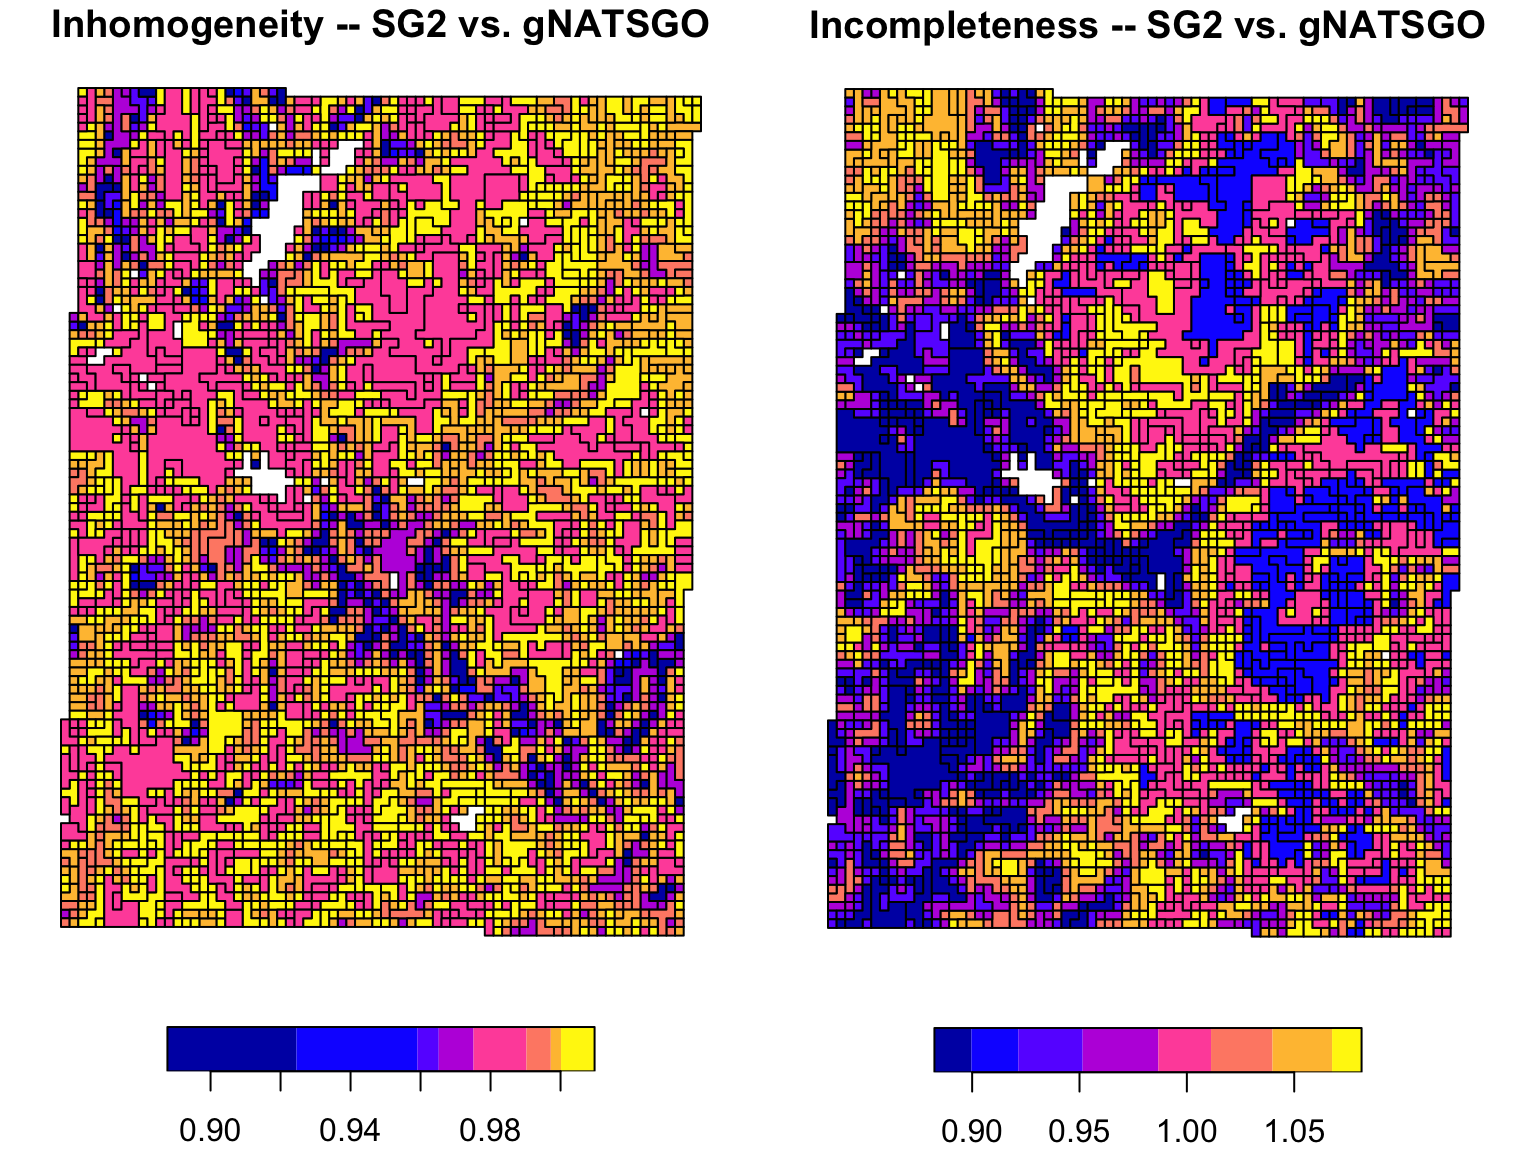
\includegraphics[height=0.72\textheight]{graphics_david/Fig16.png}
%     \end{figure}
% \end{frame}


% \begin{frame}{V-measure example}
% % latex table generated in R 4.1.2 by xtable 1.8-4 package
% 
\begin{tabular}{llll}
  \hline
DSM\hspace{1ex}products & V-measure & Homogeneity & Completeness \\ 
  \hline
gNATSGO vs.\ SG2 & 0.0128 & 0.0143 & 0.0116 \\ 
  gNATSGO vs.\ SPCG & 0.0258 & 0.0275 & 0.0243 \\ 
  gNATSGO vs.\ PSP & 0.084 & 0.0897 & 0.079 \\ 
  SPCG vs.\ SG2 & 0.3342 & 0.3495 & 0.3201 \\ 
   \hline
\end{tabular}
   
% \par
% V-measure statistics, pHx10 0--5~cm
% \end{frame}

\section{Letting the map ``speak for itself''}

\begin{frame}
  \frametitle{Finding patterns by ``letting the map speak for itself''}
  \begin{itemize}
  \item Objective: (semi-)automatically extract patterns from the map
  \item These can be compared to ``reality''
  \item Methods
    \begin{itemize}
    \item \textbf{Aggregation}: areas of ``similar'' \textbf{values} or \textbf{classes}
    \item \textbf{Segmentation}: areas with ``similar'' \textbf{internal spatial patterns}
    \end{itemize}
  \end{itemize}
\end{frame}

\begin{frame}
  \frametitle{Aggregation}
  \begin{itemize}
  \item Group grid cells (``pixels'')  of ``similar'' \textbf{values} or \textbf{classes} into ``super-pixels''
  \item R package \texttt{supercells}
  \item Parameters to control degree of similarity and how to measure it
  \end{itemize}
\end{frame}

\begin{frame}{Aggregation example -- pH class map of Tamil Nadu (part)}
    \begin{figure}
      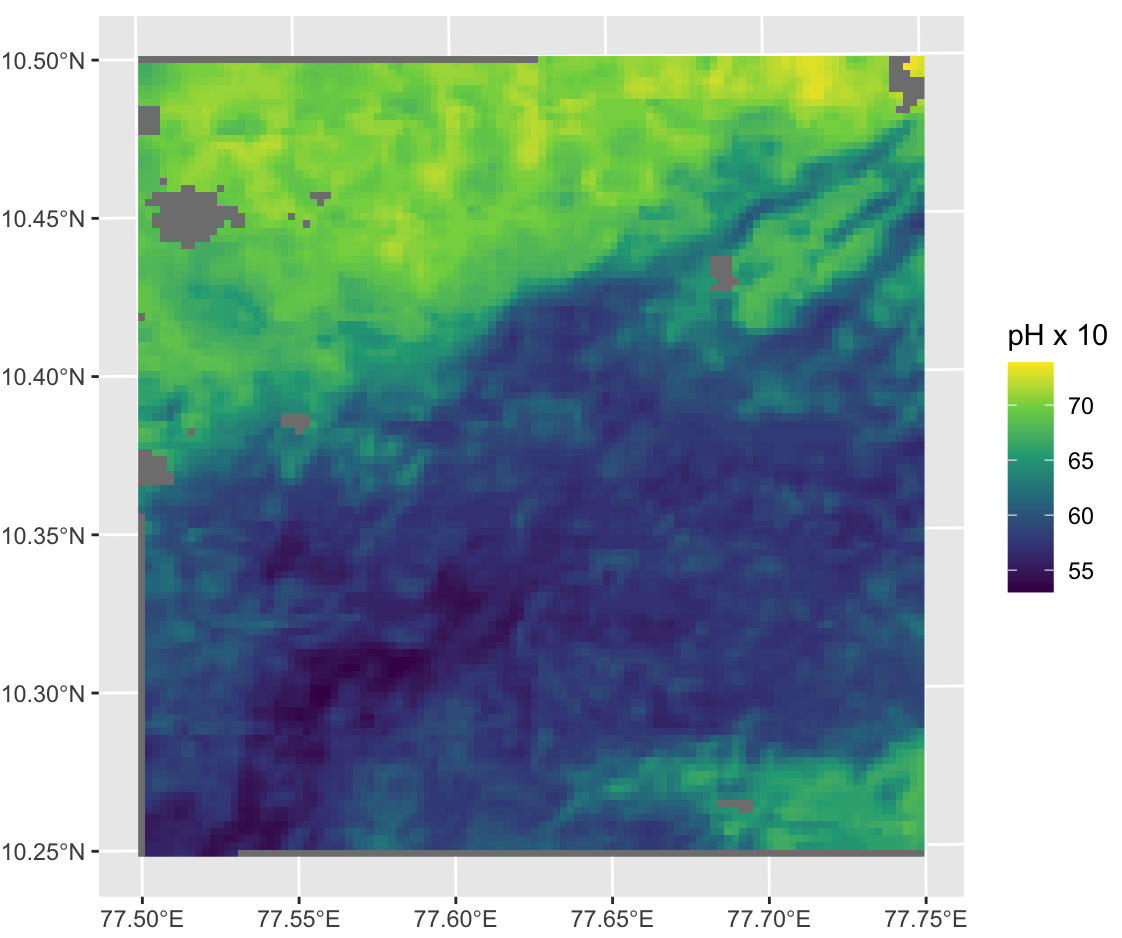
\includegraphics[width=0.45\textwidth]{graphics_david/SLIC-source-1.png}
      \hfill
      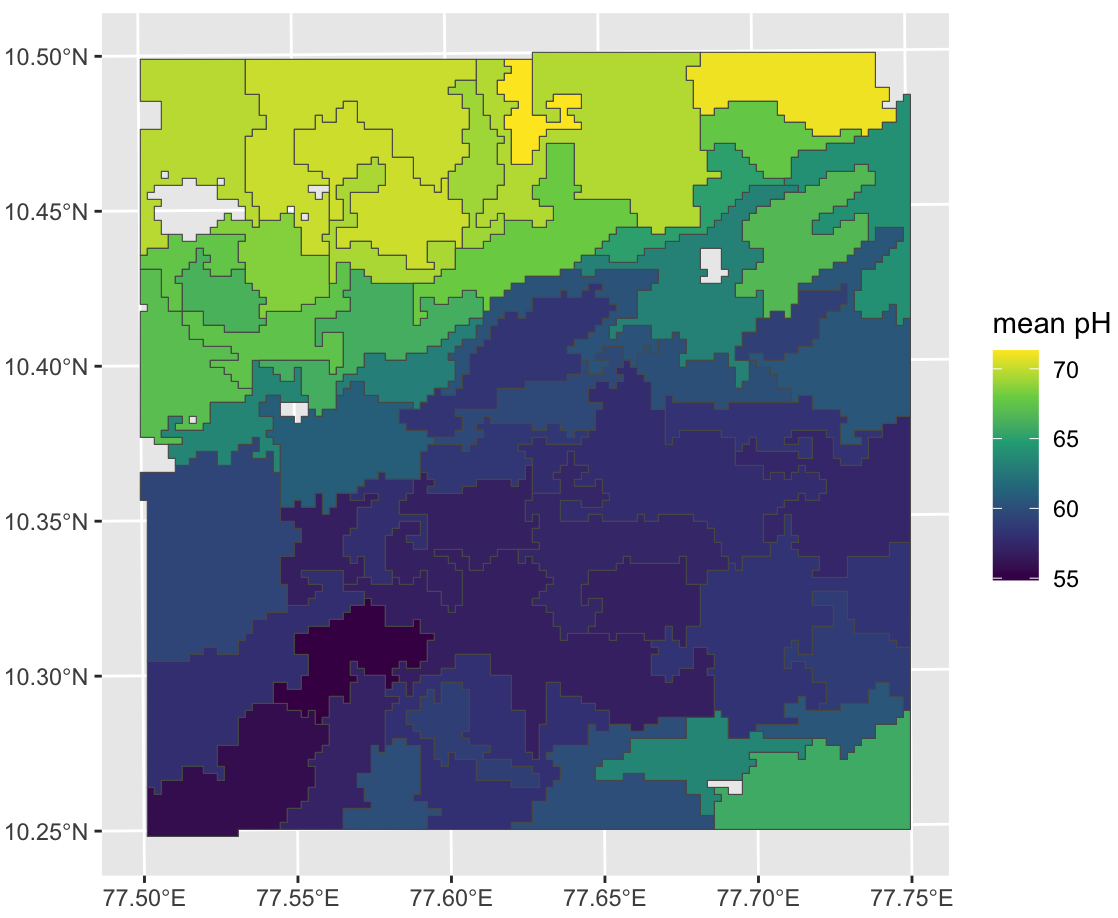
\includegraphics[width=0.45\textwidth]{graphics_david/supercells-not-compact-1.png}
    \end{figure}
    SoilGrids v.20 pH~x~10 values \hfill Supercells with mean pH~x~10
\end{frame}

% \begin{frame}{Aggregation example -- BIS-4D soil property class maps of NL}
%     \begin{figure}
%         \centering        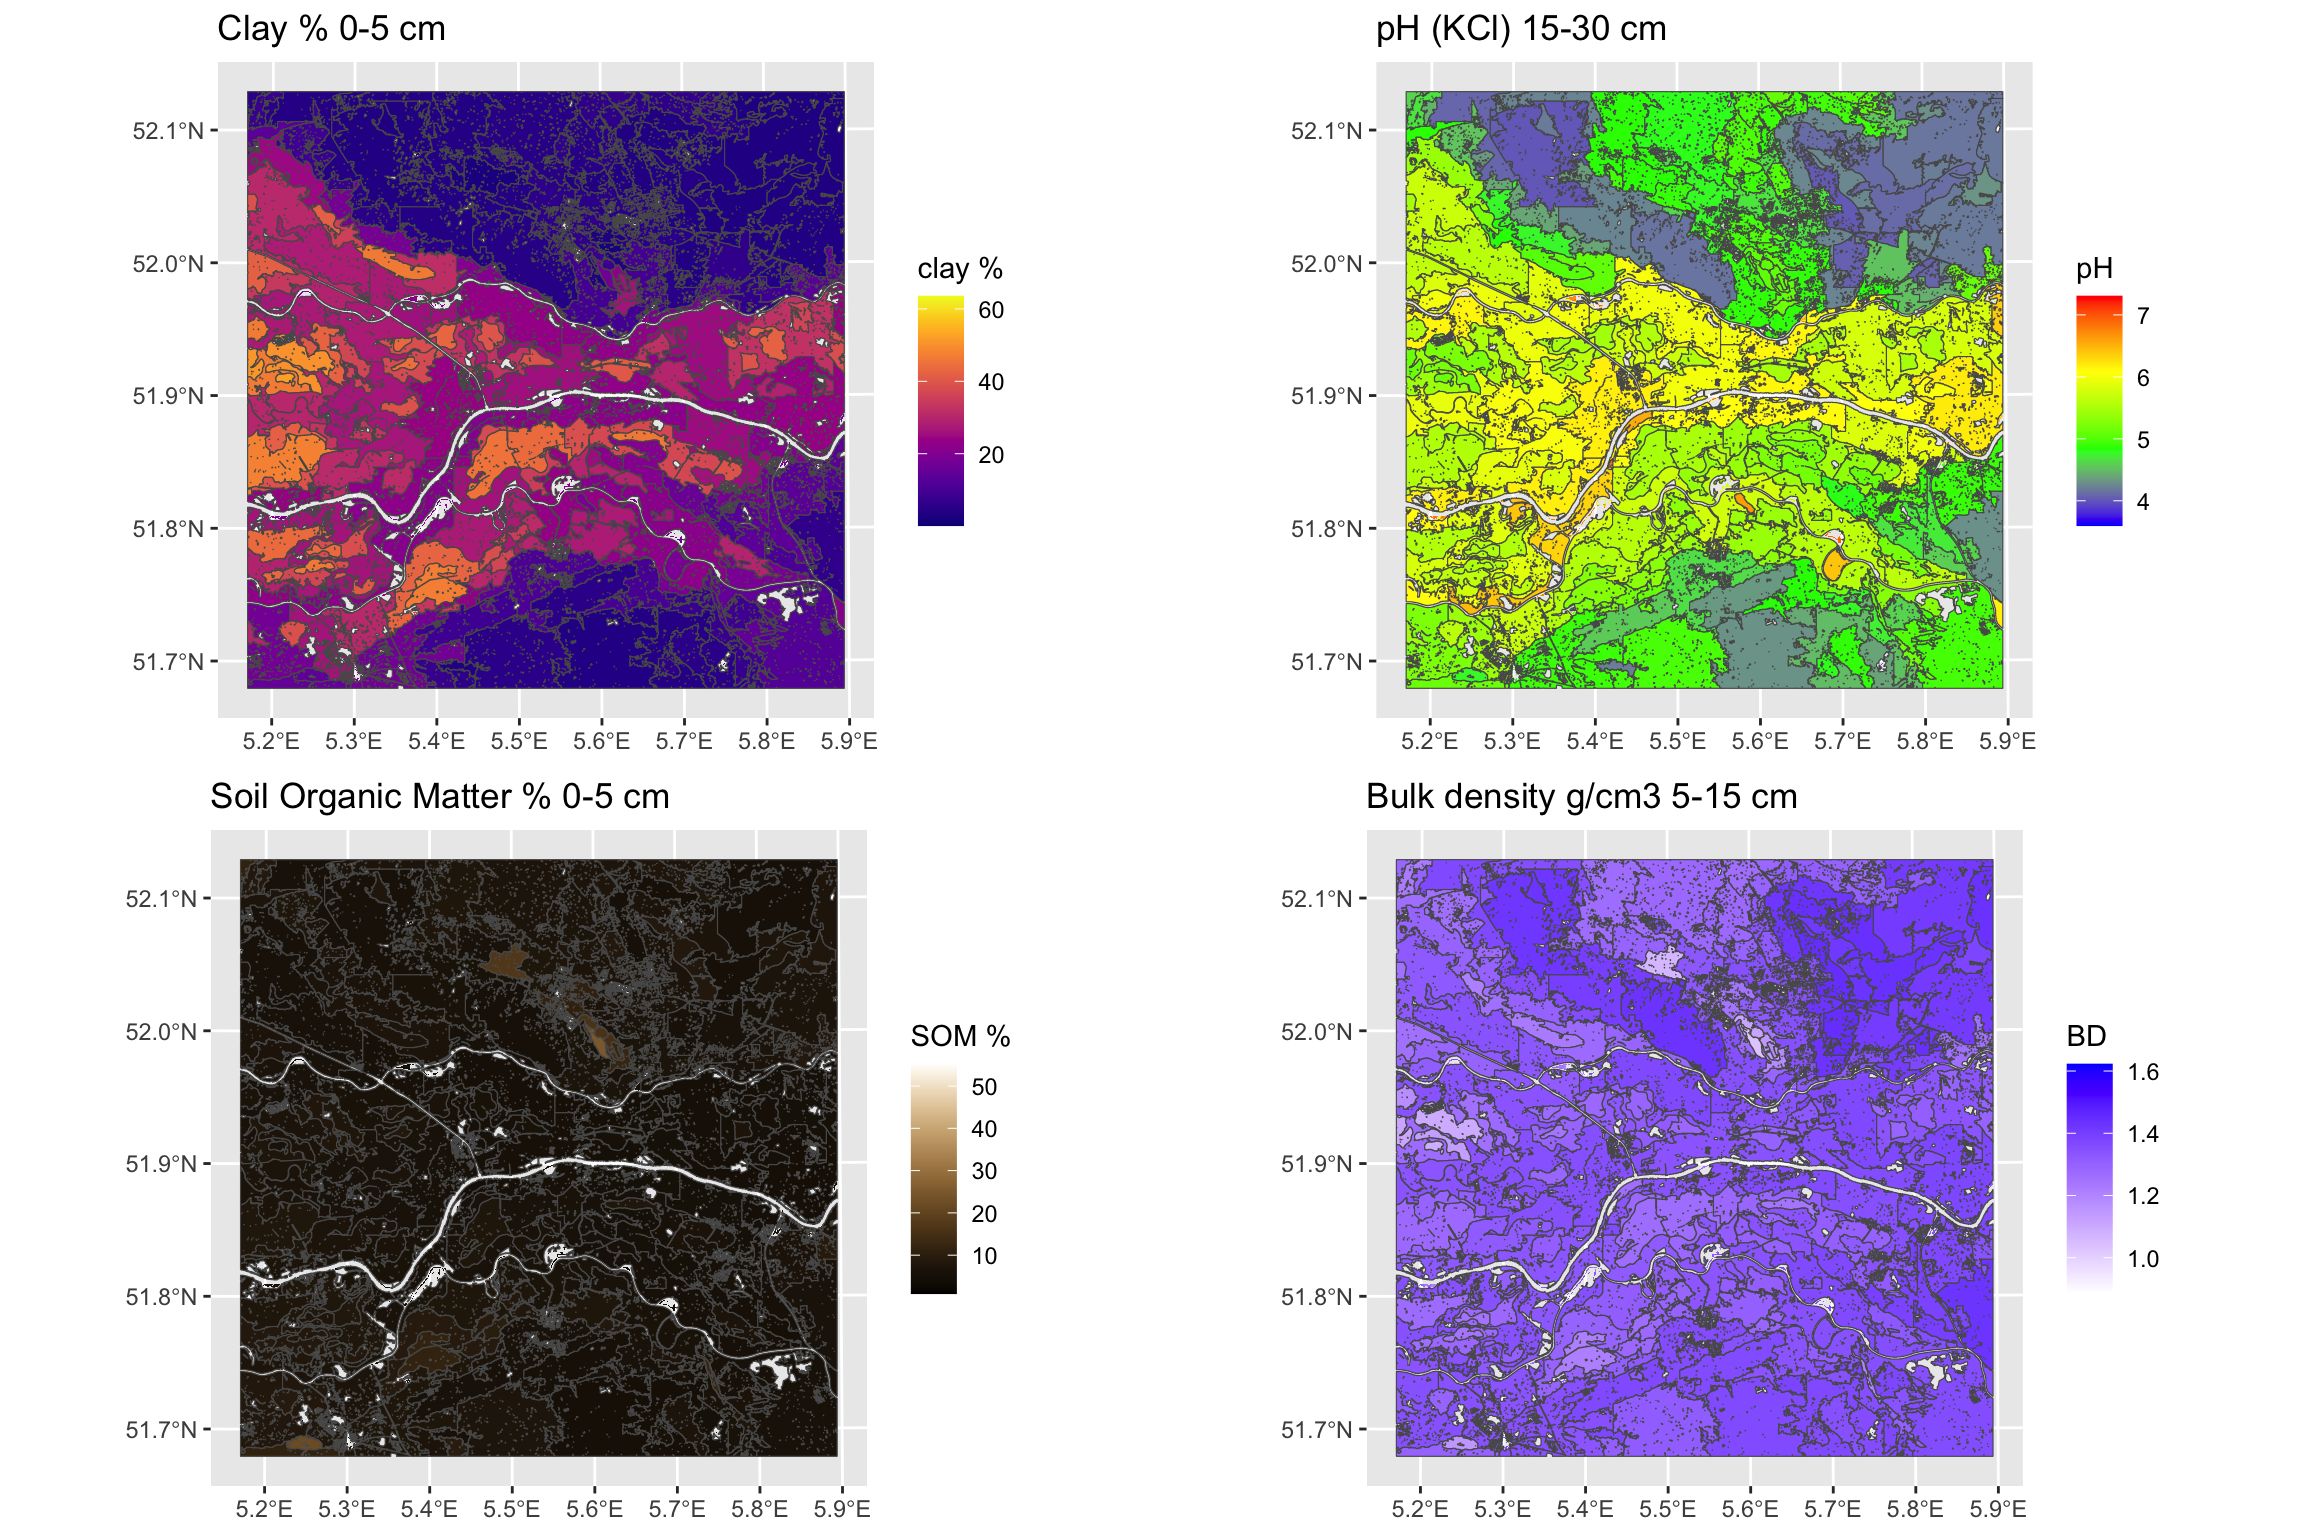
\includegraphics[height=0.70\textheight]{graphics_david/plot-supercells-bis4d-1-jsd-all-4up-1.png}
%       \end{figure}
% \end{frame}


\begin{frame}{Segmentation by patterns}
\begin{itemize}
    \item 
A recent development by Nowosad\footnote{https://jakubnowosad.com/}, based on an algorithm of Jadiewicz    
\item Aggregates groups of pixels (size set by analyst) into polygons with a ``similar enough'' spatial \textbf{pattern} of classes within the polygon
  \begin{itemize}
  \item Limitation: polygons are composed of square cells at least 10x the original grid resolution
  \end{itemize}
\item The pattern of these grid cells can be considered a \textbf{meta-pattern} of the DSM product
\end{itemize}
\end{frame}

\begin{frame}
  \frametitle{Segmentation example -- BIS-4D, bulk density of all layers}
    \begin{figure}
        \centering        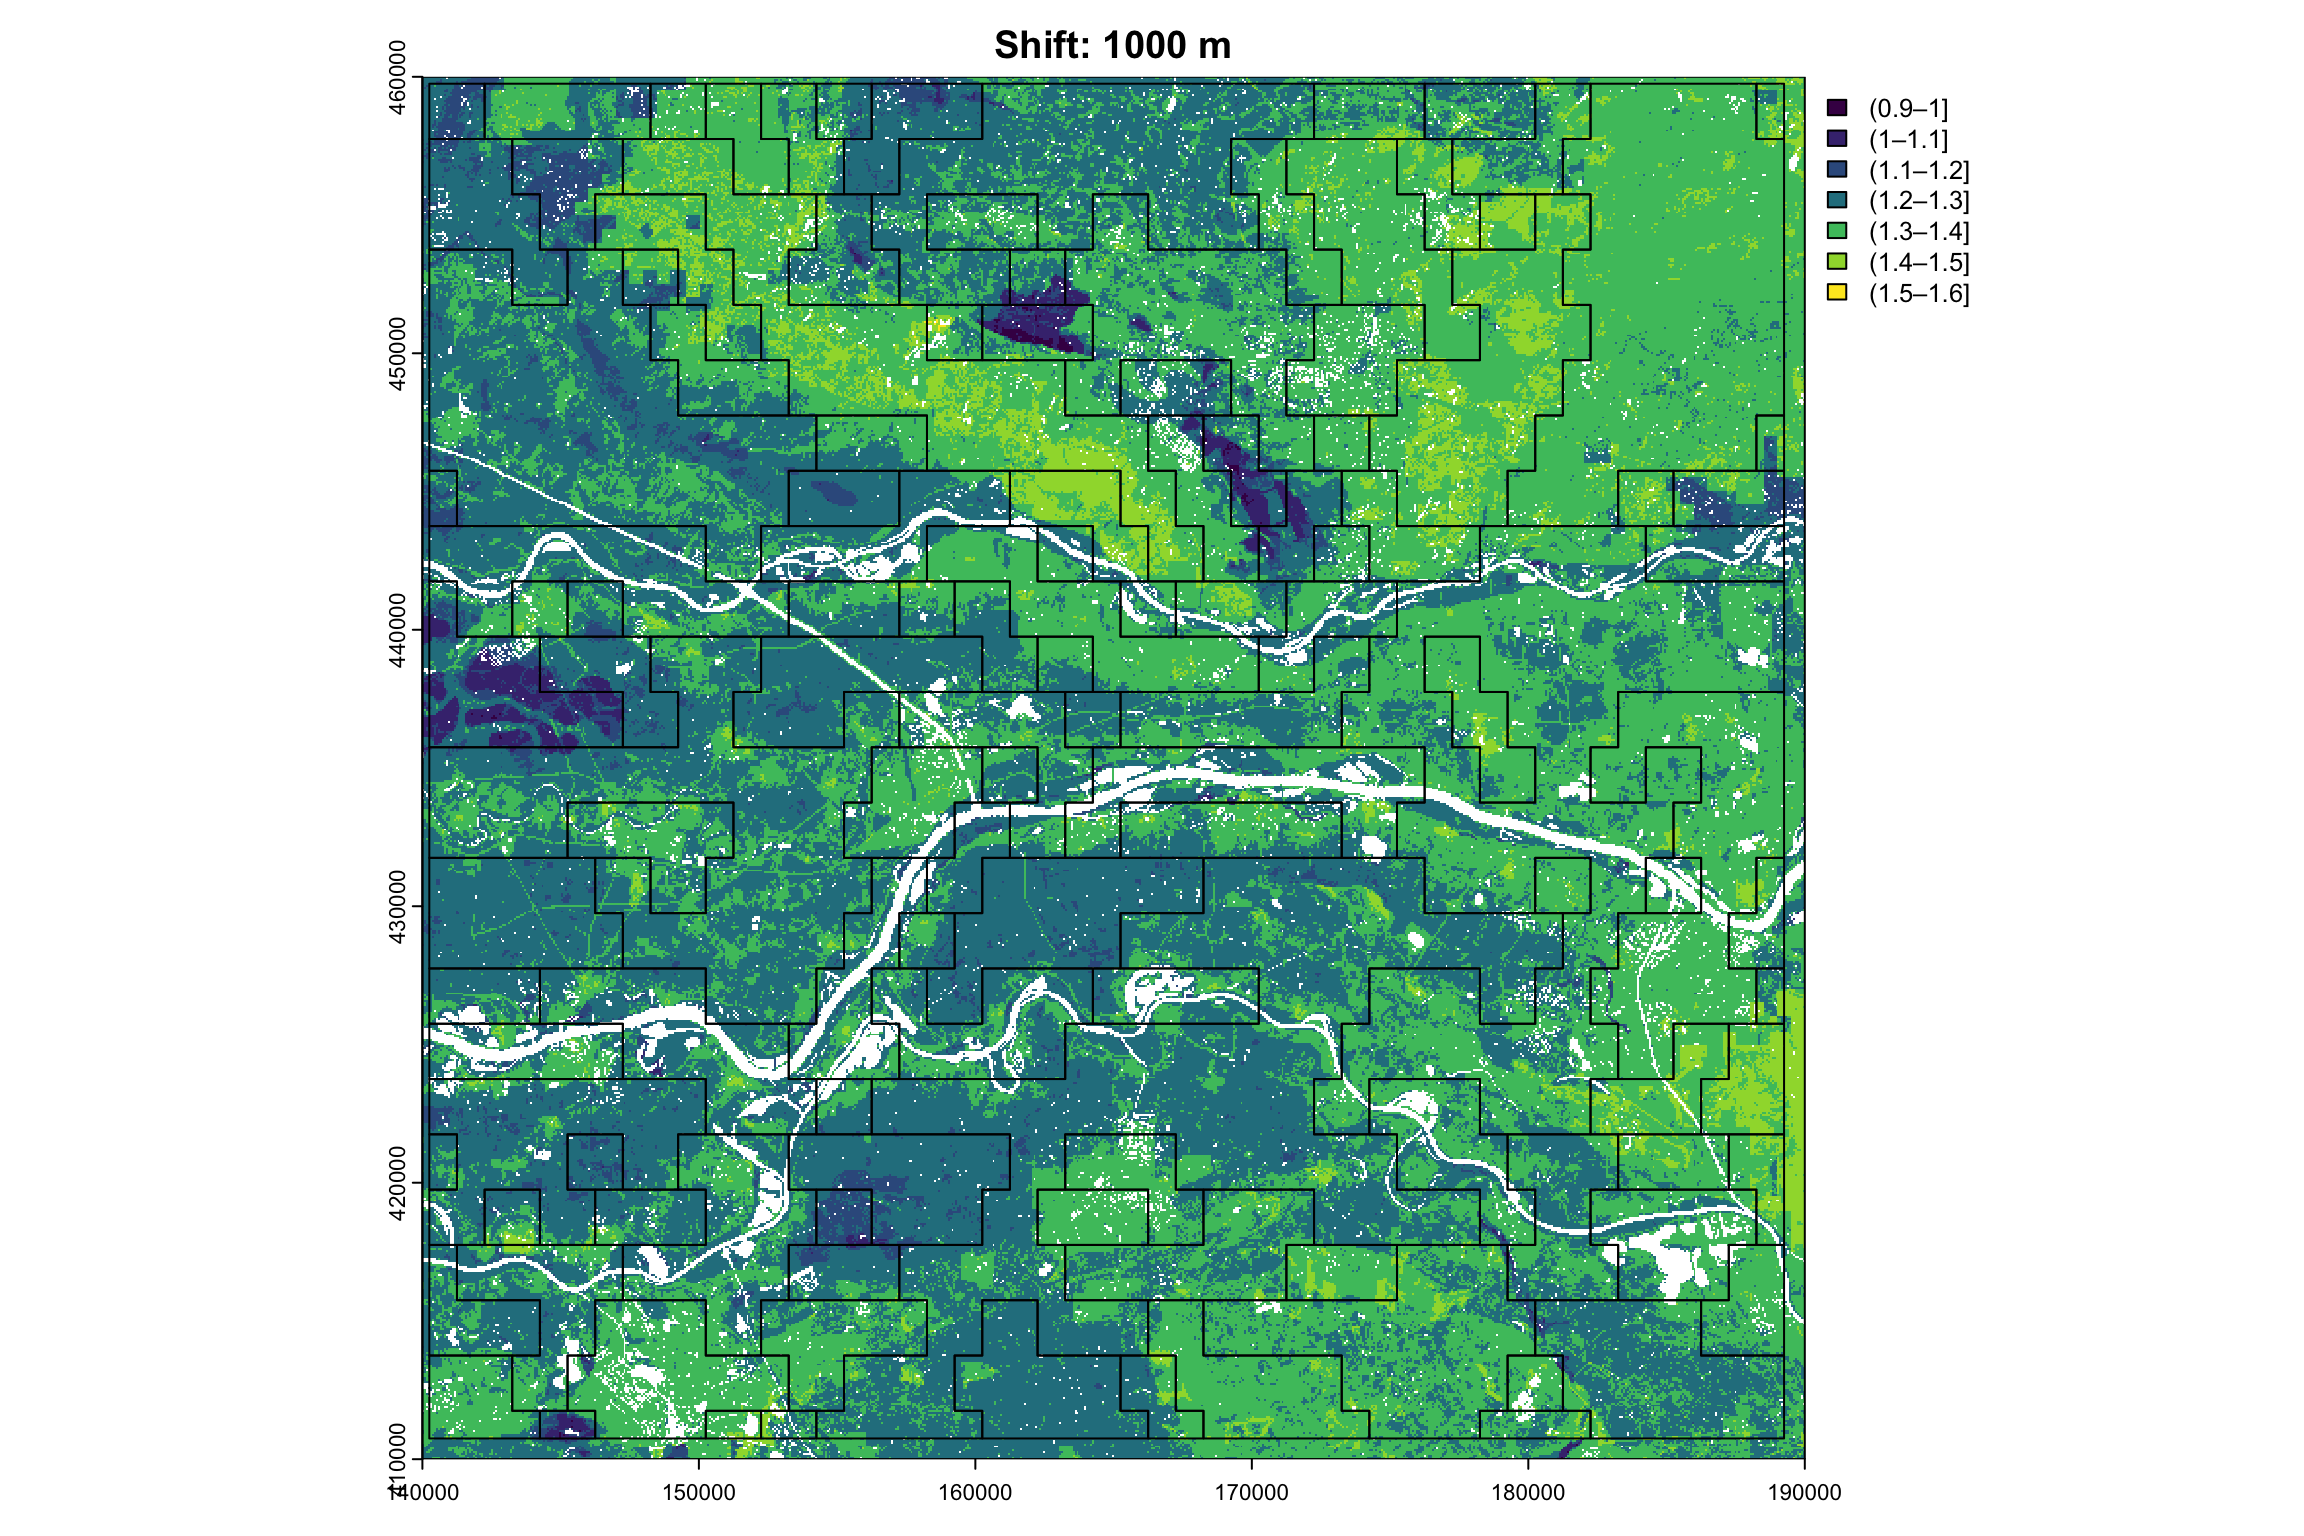
\includegraphics[height=0.7\textheight]{graphics_david/all-files-resolutions-3.png}
      \end{figure}
\end{frame}
      %
      
 % \begin{frame}
 %        \frametitle{Evaluating segmentation success}
 %    \begin{figure}
 %        \centering        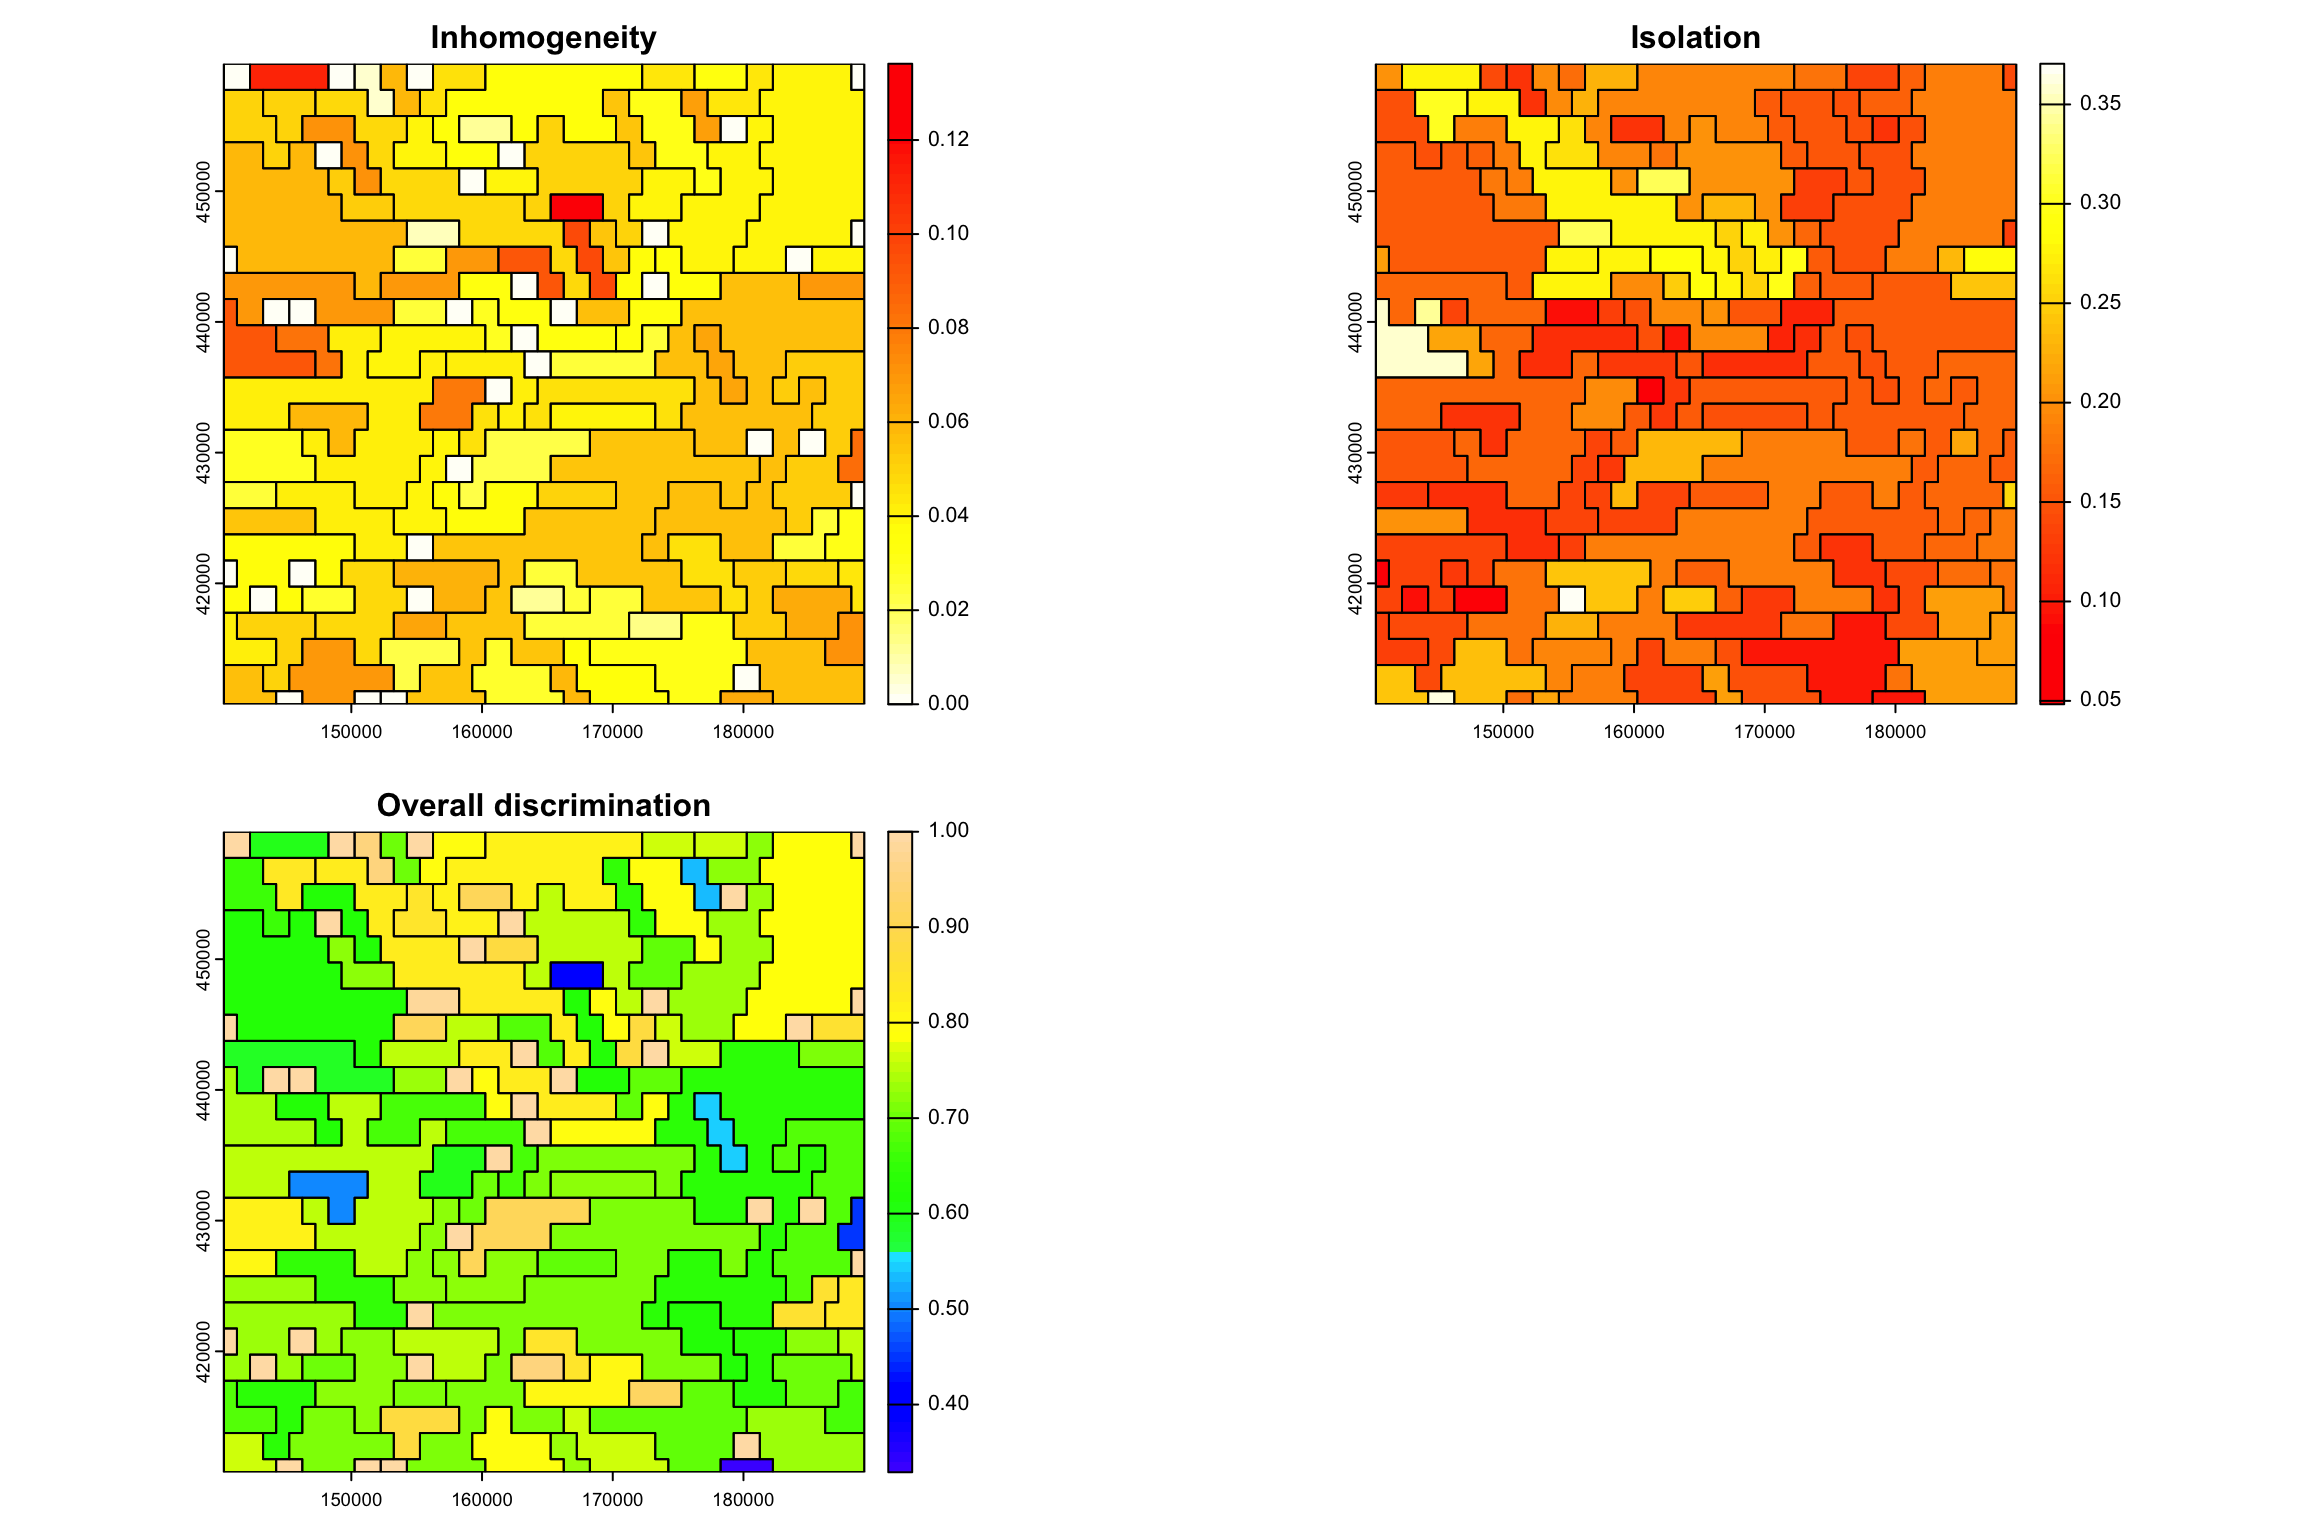
\includegraphics[height=0.7\textheight]{graphics_david/all-files-resolutions-4.png}
 %      \end{figure}
 %  \end{frame}

  \begin{frame}
    \frametitle{Characterizing the patterns in a segment}
    \begin{figure}
        \centering        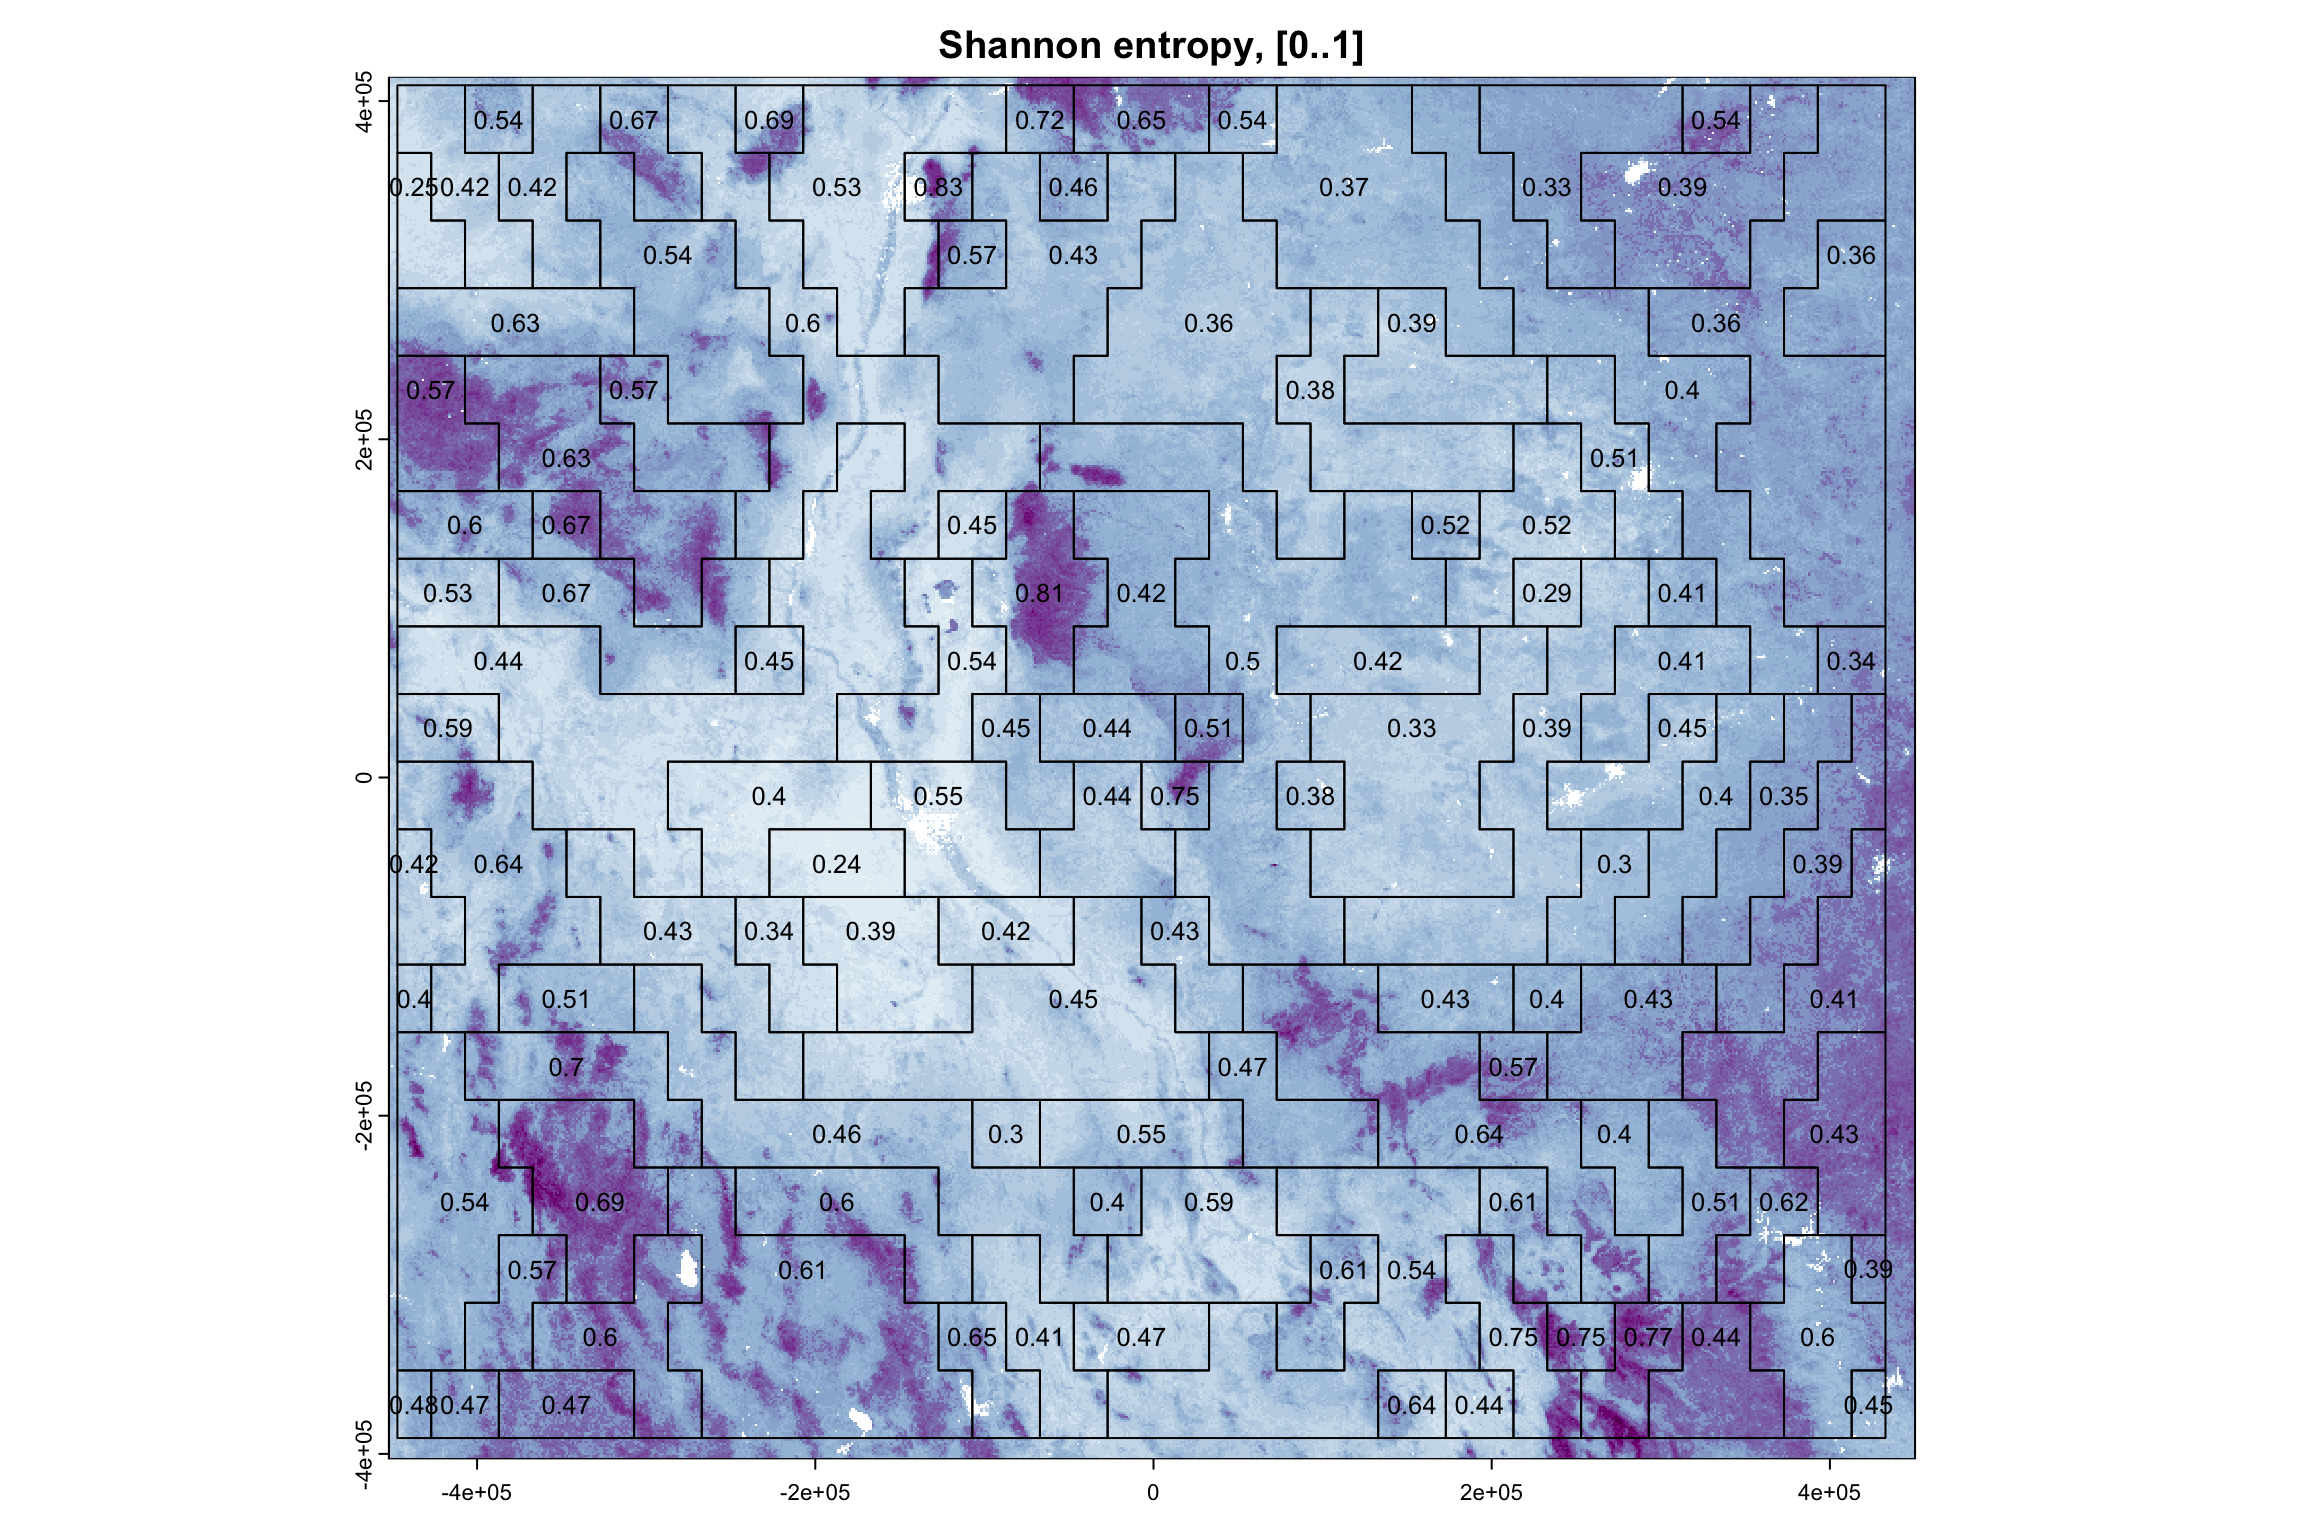
\includegraphics[height=0.6\textheight]{graphics_david/compute-sg-nm-8M-3.png}
      \end{figure}
      {\footnotesize SOC stocks predicted by SoilGrids 2.0, M\'{e}xico / USA. Centre near Alamogordo (NM)}
  \end{frame}
  
  
%\newpage
%\begin{frame}{Segmentation by patterns}
    % \begin{figure}
    %     \centering        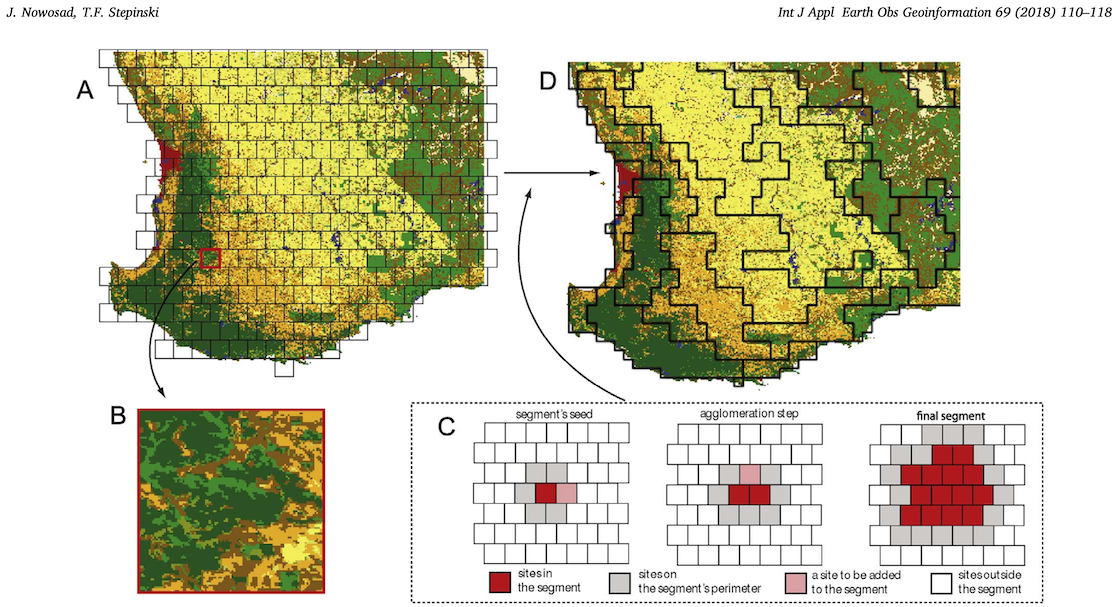
\includegraphics[height=0.9\textheight]{graphics_david/10.1016.j.jag.2018.03_Fig1.png}
    % \end{figure}
%\end{frame}

\section{Comparing maps vs.\ ``reality''}

\begin{frame}{Comparing maps; maps vs.\ ``reality''}
    \begin{itemize}
        \item The homogeneity and completeness of \textbf{one} map, representing the other, can be quantified
        \item The pattern analysis applied to \textbf{different} maps can be compared
        \item The pattern of the \textbf{difference} map can be quantified
        \item But \ldots which is closest to the \textbf{actual soil pattern} \textbf{at the design scale}?
          \begin{itemize}
          \item consider both \textbf{cartographic} and \textbf{categorical} scales
          \end{itemize}
        \item Much knowledge from traditional soil survey about actual patterns at detailed mapping scales 1:12k -- 1:50k (Fridland 1974, Hole 1978)
    \end{itemize}
\end{frame}


\begin{frame}{Scales of soil patterns}
    \begin{figure}
        \centering
        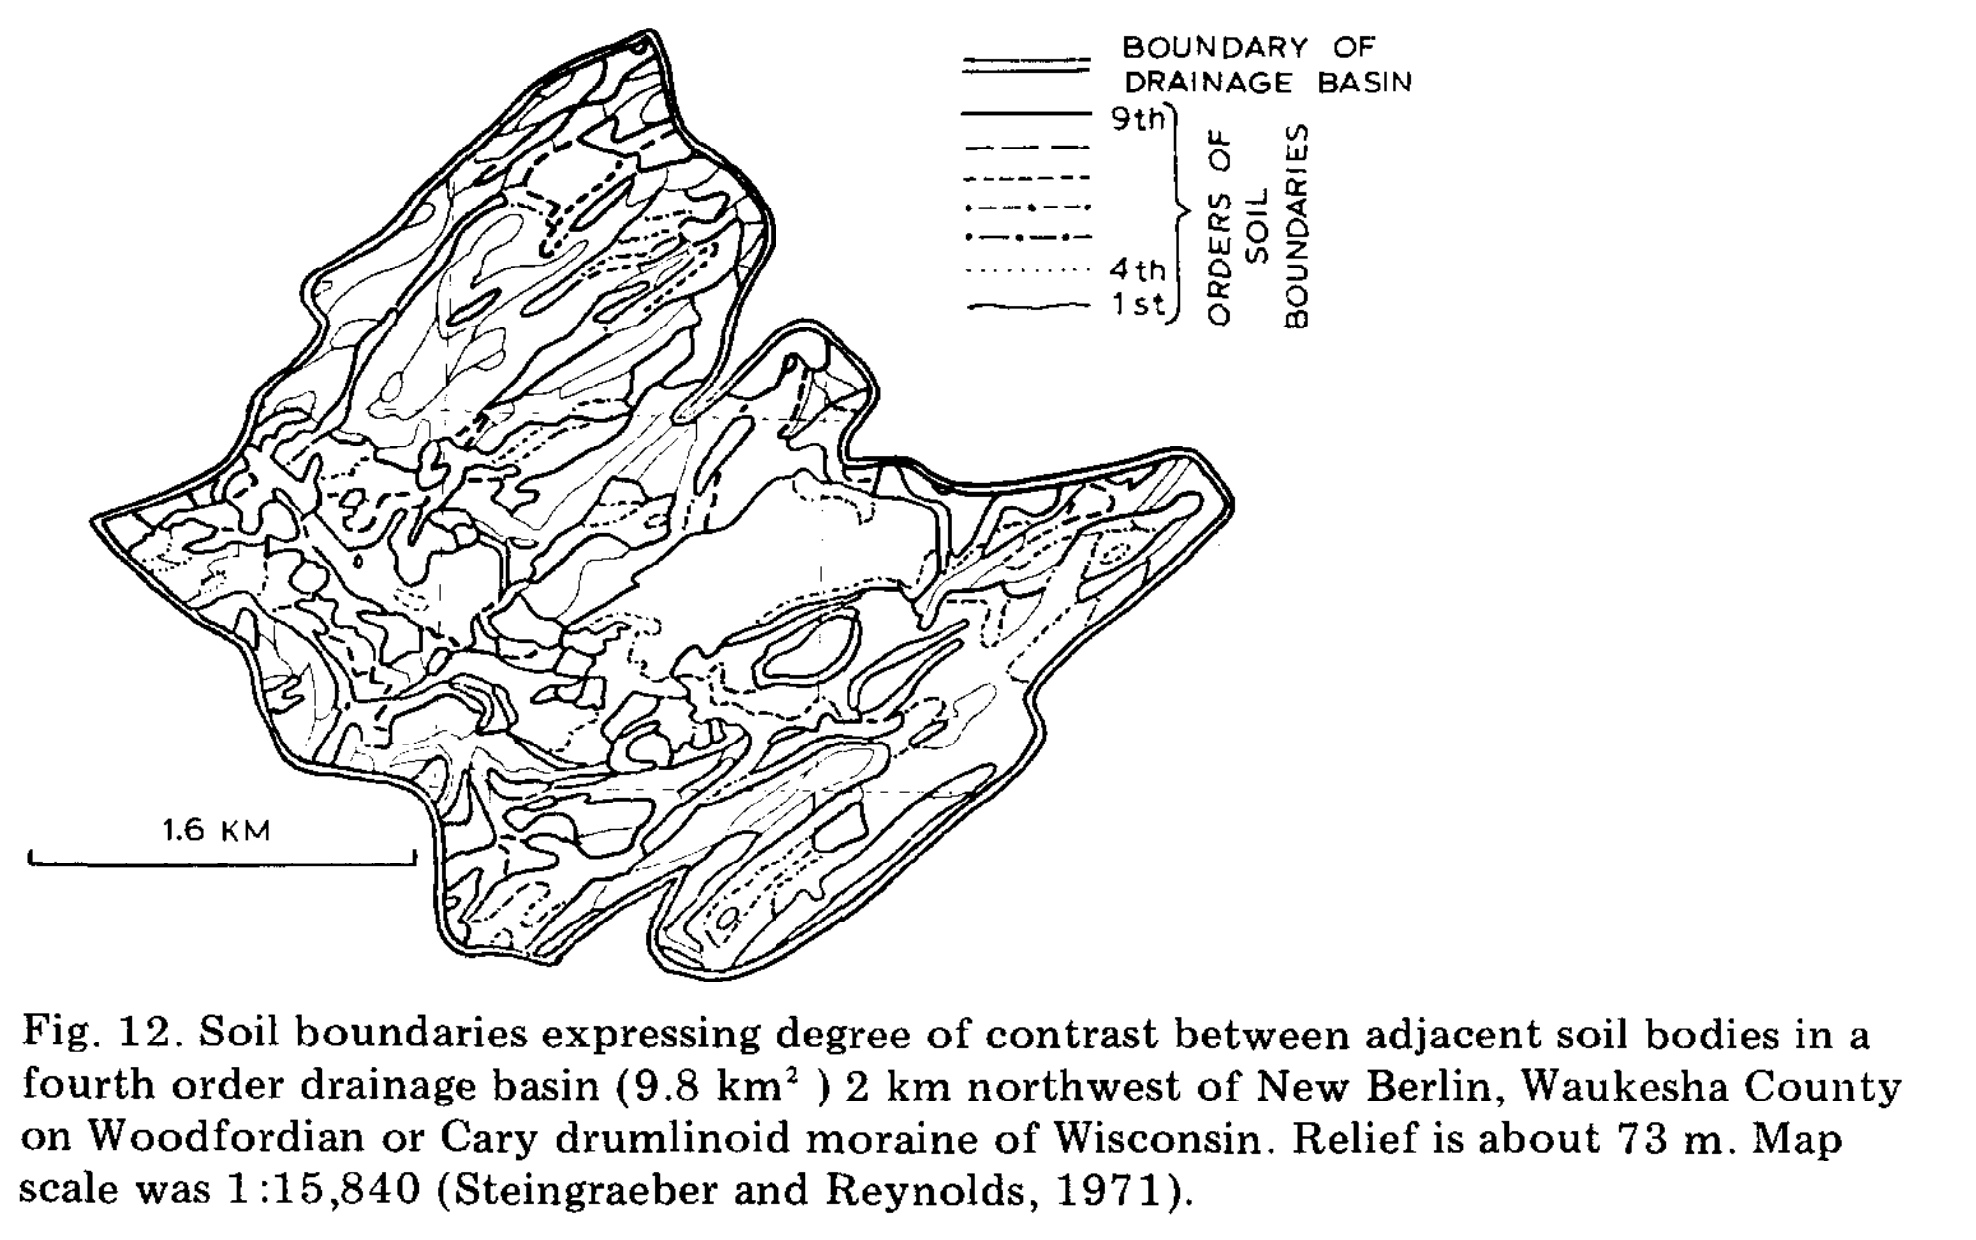
\includegraphics[height=0.75\textheight]{graphics_david/10.1016.0016-7061(78)90002-2_Fig12.png}
\\source: Hole (1978)
    \end{figure}
\end{frame}

% \begin{frame}{Resolution and scale}
% DSMaps are \textbf{gridded} at some horizontal \textbf{resolution} (``pixel size'') -- what is the relation to map scale?
% \\[2ex]
%     \begin{figure}
%     \centering
% 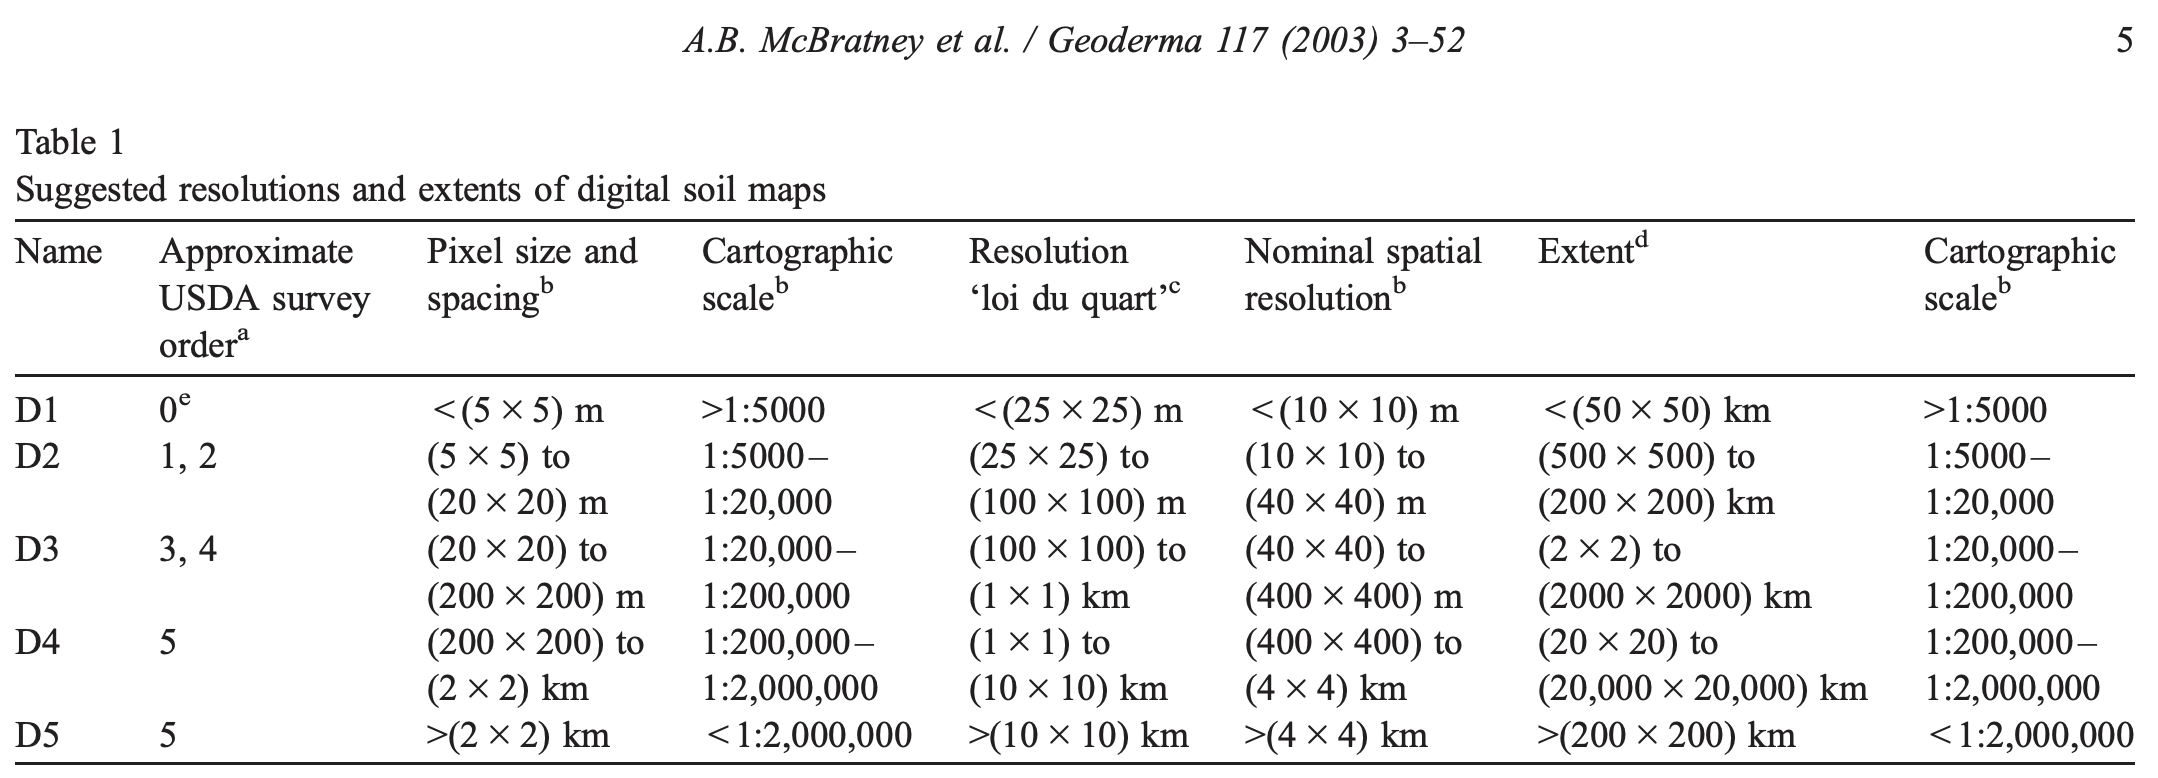
\includegraphics[width=\textwidth]{./graphics_david/McBratney2013_Table1.png}
% \end{figure}
% \end{frame}

\begin{frame}
  \frametitle{DSM scale effects -- 20 vs.\ 250~m resolution gSSURGO}
    \begin{figure}
    \centering
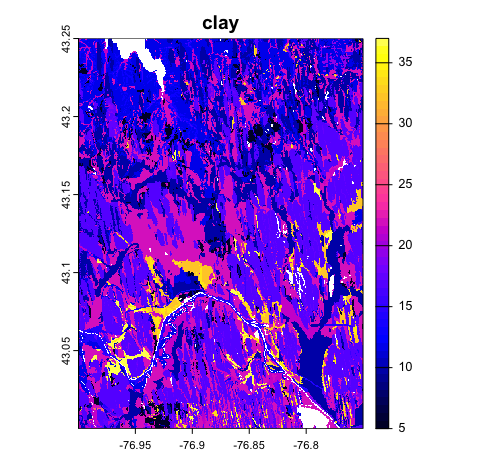
\includegraphics[width=0.45\textwidth]{./graphics_david/ClydeNY_gSSURGO_20.png}
\hfill
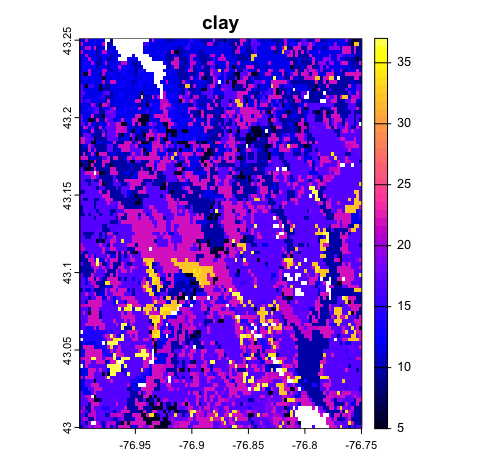
\includegraphics[width=0.45\textwidth]{./graphics_david/ClydeNY_gSSURGO_250.png}
\end{figure}  
\end{frame}

% \begin{frame}{What will the map be used for?}
%     \begin{itemize}
%         \item This governs the selection of grid cell size.
%         \item The soil variability \emph{within} the grid cell is ignored \ldots
%         \begin{itemize}
%             \item \ldots for the map user \ldots
%             \item so, for the evaluator
%         \end{itemize}
%         \item The \textbf{single value} of the grid cell represents the value the user will put in their ``model''
%         \item The \textbf{uncertainty} of the grid cell is the uncertainty \textbf{of that predicted value}, \emph{not} the variance within the grid cell.
%     \end{itemize}
% \end{frame}

\begin{frame}{Should the DSM match the polygon map?}
    \begin{itemize}
        \item Maybe DSM finds the ``inclusions'' within the map unit polygon
        \item This depends on the DSM resolution vs.\ minimum legible delineation (MLD) derived from the design scale
        \begin{itemize}
            \item $0.4~\mathrm{cm}^2$ on map $\to$ ground area
            \item e.g., 1:24k $\to$ MLD 2.3~ha; 1:12k $\to$ 0.576~ha
            \item If 4 pixels per MLD, pixel resolution 96~m (1:24k), 48~m (1:12k)
        \end{itemize}
        \item There is no way to check this spatially, but the proportion can be compared to estimates
    \end{itemize}
  \end{frame}
  
\section{On, on!}

\begin{frame}{Next steps}
\begin{enumerate}
    \item Publish paper on ``letting the map speak for itself''
    \item Match metrics with soil patterns at various scales and in various soil-landscapes
    \item Quantify these matches
\end{enumerate}
\end{frame}


%----------------
% Closing frame

\setbeamertemplate{background}{
\includegraphics[width=\paperwidth,height=\paperheight]{background_end.png}}
\setbeamertemplate{footline}{} % no footer on title

  \begin{frame} 
    \frametitle{}
    \framesubtitle{}

 \begin{center}
 \vspace{0.5cm}
 \textcolor{isric_yellow}{\Large{Questions, comments, ideas, suggestions?}}
 \end{center}
 \textcolor{isric_yellow}{e-mail: \url{david.rossiter@isric.org}}
  \\
  \textcolor{isric_yellow}{www: \url{https://www.css.cornell.edu/faculty/dgr2/index.html}}
\end{frame} 


\setbeamertemplate{background}{

\includegraphics[width=\paperwidth,height=\paperheight]{background_slides.png}}

\setbeamertemplate{footline}[eawag] % set footer

\begin{frame}[allowframebreaks]{References}

  \begin{scriptsize}
\begin{itemize}

  % \item Bohn, M. P., \& Miller, B. A. (2024). Locally enhanced digital soil mapping in support of a bottom-up approach is more accurate than conventional soil mapping and top-down digital soil mapping. Geoderma, 442, 116781. \url{https://doi.org/10.1016/j.geoderma.2024.116781}

    \item Boulaine, J. (1982). Remarques sur quelques notions élémentaires de la pédologie. Cahiers O.R.S.T.O.M., série Pédologie, 19(1), 29-41.

      % \item Eymard, A., Richer-de-Forges, \ldots \& Arrouays, D. (2024). Exploring the untapped potential of hand-feel soil texture data for enhancing digital soil mapping: Revealing hidden spatial patterns from field observations. Geoderma, 441, 116769. \url{https://doi.org/10.1016/j.geoderma.2023.116769}
 
    \item Fridland, V. M. (1974). Structure of the soil mantle. Geoderma, 12, 35-42. \url{https://doi.org/10.1016/0016-7061(74)90036-6}

    \item Hole, F. D. (1978). An approach to landscape analysis with emphasis on soils. Geoderma, 21(1), 1-23. \url{https://doi.org/10.1016/0016-7061(78)90002-2}

    \item Hudson, B. D. (1992). The soil survey as paradigm-based science. Soil Science Society of America Journal, 56(3), 836-841. \url{https://doi.org/0.2136/sssaj1992.03615995005600030027x}

    \item Jasiewicz, J., Netzel, P., \& Stepinski, T. (2015). GeoPAT: A toolbox for pattern-based information retrieval from large geospatial databases. Computers \& Geosciences, 80, 62-73. \url{https://doi.org/10.1016/j.cageo.2015.04.002}

    \item Lagacherie, P., Andrieux, P., \& Bouzigues, R. (1996). Fuzziness and uncertainty of soil boundaries: From reality to coding in GIS. In P. A. Burrough, A. U. Frank, \& F. Salgé (Red.), Geographic objects with indeterminate boundaries (pp. 275-286). Taylor \& Francis.

    \item McBratney, A. B., Mendon\c{c}a Santos, M. L., \& Minasny, B. (2003). On digital soil mapping. Geoderma, 117(1-2), 3-52. \url{https://doi.org/10.1016/S0016-7061(03)00223-4}

    \item Nowosad, J. (2021). Motif: An open-source R tool for pattern-based spatial analysis. Landscape Ecology, 36(1), 29-43. \url{https://doi.org/10.1007/s10980-020-01135-0}

    
    \item Nowosad, J., \& Stepinski, T. F. (2018). Towards machine ecoregionalization of Earth’s landmass using pattern segmentation method. International Journal of Applied Earth Observation and Geoinformation, 69, 110-118. \url{https://doi.org/10.1016/j.jag.2018.03.004}

    \item Poggio, L., de Sousa, L. M., Batjes, N. H., Heuvelink, G. B. M., Kempen, B., Ribeiro, E., \& Rossiter, D. (2021). SoilGrids 2.0: Producing soil information for the globe with quantified spatial uncertainty. SOIL, 7(1), 217--240. \url{https://doi.org/10.5194/soil-7-217-2021}

    % \item Riitters, K. H., Vogt, P., Soille, P., Kozak, J., \& Estreguil, C. (2007). Neutral model analysis of landscape patterns from mathematical morphology. Landscape Ecology, 22(7), 1033-1043. \url{https://doi.org/10.1007/s10980-007-9089-3}

    % \item Riitters, K., Vogt, P., Soille, P., \& Estreguil, C. (2009). Landscape patterns from mathematical morphology on maps with contagion. Landscape Ecology, 24(5), 699-709. \url{https://doi.org/10.1007/s10980-009-9344-x}

    \item Rossiter, D. G., Poggio, L., Beaudette, D., \& Libohova, Z. (2022). How well does digital soil mapping represent soil geography? An investigation from the USA. SOIL, 8(2), 559--586. \url{https://doi.org/10.5194/soil-8-559-2022}

    % \item Sciaini, M., Fritsch, M., Scherer, C., \& Simpkins, C. E. (2018). NLMR and landscapetools: An integrated environment for simulating and modifying neutral landscape models in R. Methods in Ecology and Evolution, 9(11), 2240-2248.\url{https://doi.org/10.1111/2041-210X.13076}

      \item Yang, L., Jiao, Y., Fahmy, S., Zhu, A.-X., Hann, S., Burt, J. E., \& Qi, F. (2011). Updating conventional soil maps through digital soil mapping. Soil Science Society of America Journal, 75(3), 1044-1053. \url{https://doi.org/10.2136/sssaj2010.0002}

    \end{itemize}
  \end{scriptsize}
\end{frame}

%----------------
\end {document}

%  LocalWords:  setbeamertemplate paperwidth,height paperheight eawag
%  LocalWords:  addtocounter framenumber geostatistical textit pedons
%  LocalWords:  varepsilon flushleft Boulaine Soilscape Lagacherie
%  LocalWords:  Otsego textdegree textdegree landscapemetrics rassta
%  LocalWords:  Variogram Variograms discretize equalization shdi
%  LocalWords:  characterizes summarizes normalized shei Nowosad
%  LocalWords:  landscape_metrics_lat4243_lon-77-76_phh2o_0-5 Eymard
%  LocalWords:  Stepinski Jadiewicz framesubtitle isric_yellow Salgé
%  LocalWords:  compare_vmeasure_lat4243_lon-77-76_phh2o_0-5 Geoderma
%  LocalWords:  allowframebreaks Arrouays Burrough Minasny
